\chapter{Evolución en la propuesta \color{red}(In progress)\color{black}}

En este capítulo se realizará un análisis completo paso por paso del proceso de desarrollo del algoritmo. 
Se mostrarán distintas tablas y gráficas comparativas y sus interpretaciones con el fin de justificar la motivación de las distintas modificaciones introducidas explicadas en el capítulo anterior.

\section{Diseño Experimental}
\subsection{Criterio de Parada}

Se han elegido las instancias mencionadas anteriormente (\href{http://cedric.cnam.fr/~soutif/QKP/QKP.html}{(QKP) \textit{instances}}) ya que también se proporcionaban algunos resultados de otros algoritmos, por lo que resultaba conveniente a la hora de comprobar si los resultados obtenidos por nuestros algoritmos bases eran competitivos. 
Ya que, en el caso de que no lo fuesen, tendríamos que buscar otros algoritmos base sobre los que trabajar.
Sin embargo, nos encontramos con un problema, esto es, el criterio de parada presentado en estos casos es el tiempo.
Adicionalmente, el tiempo de parada también depende del número de elementos, $n$, de forma que se tiene:
\begin{itemize}
\item Para $n = 100$, se tienen \textbf{5 segundos} de ejecución.
\item Para $n > 100$, en nuestro caso, $n = 200$ y $n = 300$, se tienen \textbf{30 segundos} de ejecución.
\end{itemize}

Como se ha indicado antes, utilizar el tiempo de ejecución como criterio de parada resulta un problema. 
Esto se debe a que no es un criterio de parada fiable, ya que depende de la capacidad de computación de cada ordenador. 
No es comparable la velocidad de los ordenadores actuales con la velocidad de los ordenadores de dentro de 10 años, de la misma no podemos comparar el rendimiento de un ordenador de hace 10 años con respecto a uno actual. 
E incluso dentro de los ordenadores de la misma generación, dependerá de las características propias de cada computador. 
Por lo que se llega a la conclusión de que si se quiere que los resultados obtenidos en este trabajo puedan ser usados como referencia, o incluso si se quiere recrear el trabajo, en un futuro se debe cambiar el criterio de parada a algo portable, a algo que sea independiente de cuándo se produzca el experimento. 
Por ello, se ha decidido cambiar el criterio de parada a un número de iteraciones máximo. 
Este criterio sí es portable, ya que independientemente de qué tipo de computador se utilice para obtener los resultados siempre se van a obtener los mismos resultados utilizando los mismos parámetros.

Primero debemos indicar lo que entenderemos por iteraciones. 
Denotaremos como iteraciones al número de veces que se repite el procedimiento completo un determinado algoritmo, en nuestro caso se va a traducir en lo siguiente: 
\begin{itemize}
	\item Para el algoritmo \textit{Random}, el número iteraciones será el número de veces que generemos una solución de forma aleatoria.
	\item Para los algoritmos genéticos, una iteración puede suponer un número distinto de evaluaciones. 
	En los algoritmos genéticos al número de iteraciones se llama también generaciones.
\end{itemize}

Dicho esto, para elegir el número de iteraciones máximo que se iba a utilizar se tomó como referencia el tiempo establecido anteriormente. 
En tanto se tenía elegir un número de iteraciones como criterio de parada, se decidió estudiar a qué equivalía actualmente el criterio de parada por tiempo establecido. 
Para ello, mediante una variable \texttt{contador}, se ejecutaron todos los archivos con el tiempo como criterio de parada y se mostraba por pantalla el número de iteraciones que se había alcanzado. 
Tras realizar una media de todos estos datos y redondearlo, obtenemos que el nuevo criterio de parada es \textbf{90000 iteraciones} para todos los archivos. 
El que el número de iteraciones máximo no dependa del número de elementos como lo hacía el tiempo de ejecución máximo se puede justificar en tanto que se necesita más tiempo para realizar todos los cálculos si aumenta el número de datos. 

Además, para asegurarnos que realmente ambos criterios de parada eran equivalentes, se ejecutaron todos los archivos usando el algoritmo base con criterio de parada por iteraciones y por tiempo. 
Nótese que no solo se almacenan las soluciones finales, si no que también se almacenan las soluciones intermedias llegado a ciertos porcentajes de la ejecución. 
Tras esto, se compararon ambos resultados y se pudo comprobar que, efectivamente, eran equivalentes. 

Por lo tanto, se puede decir con seguridad que los cambios que apliquemos a un criterio de parada en específico se puede traducir a un cambio en el otro criterio de parada. 
Esto cabe la pena destacarlo ya que, recordemos, el objetivo de este trabajo es crear un algoritmo útil y competitivo para tratar con problemas \textit{expensive}, por lo que queremos obtener buenos resultados en un tiempo muy reducido. 

Para simular de forma eficiente y suficiente esta reducción de tiempo, se propuso el siguiente cambio con respecto al tiempo como criterio de parada:
\begin{itemize}
	\item En vez de ejecutar los archivos con $n=100$ durante 5 segundos, lo reduciremos a 25ms.
	\item En vez de ejecutar los archivos con $n>100$ durante 30 segundos, lo reduciremos a 150ms.
\end{itemize}
Realizamos un cálculo básico para comprobar qué proporción de la ejecución estaremos realizando con estos nuevos tiempos:
\begin{equation*}
\dfrac{25\cdot 100ms}{5\cdot 1000ms} = 0.5
\hspace{1cm}
\dfrac{150\cdot 100ms}{30\cdot 1000ms} = 0.5
\end{equation*}
Por lo tanto, obtenemos que solo utilizaremos el 0.5\% inicial de cada ejecución, lo que podemos traducir en que nuestro nuevo criterio de parada serán \textbf{450 iteraciones}. 

Con el fin de comprobar que esta reducción había sido suficiente y necesaria, se ejecutan de nuevo todos los archivos con el algoritmo base ahora con 450 iteraciones y comparamos los resultados con los obtenidos anteriormente con 90000 iteraciones. 
Podemos ver que, efectivamente, se han obtenido resultados mucho peores. 

Finalmente, ya hemos establecido nuestro criterio de parada escalable y tenemos unos resultados base que utilizar. 
A partir de esto, nuestro objetivo será mejorar estos resultados lo máximo posible.

\subsection{Parámetros}

La ejecución del programa no requiere de la introducción manual de ningún tipo de parámetro. 
Todos los parámetros que se nombren a continuación vienen definidos dentro del código del programa \texttt{main} como constantes globales o que dependen del propio problema. 

En primer lugar, recordemos brevemente los parámetros que utilizaremos y sus valores. 
Estos parámetros no necesitan ser introducidos manualmente al ejecutar el programa, si no que están definidos como constantes en el código:

\begin{itemize}
	\item \texttt{NEVALUACIONESMAX}: Es el número de iteraciones máximas, mantendremos su valor a 450 por lo explicado en el apartado anterior. 
	\item \texttt{NTRIES}: Para eliminar la aleatoriedad que proviene de la ejecución con una determinada semilla u otra, cada algoritmo se ejecutará \texttt{NTRIES} número de veces, haremos la media de sus ejecuciones y este valor será el resultado que se guardará y se comparará posteriormente con el resto. 
	Para que los resultados puedan ser comparados estadísticamente, pero a la vez se mantenga un tiempo de ejecución razonable, estableceremos su valor a 50.
	\item \texttt{INITSEED}: En relación con la constante anterior, es necesario no utilizar siempre la misma semilla de aleatoriedad, ya que eso resultaría en obtener siempre los mismos resultados, por lo que ejecutarlos varias veces sería una pérdida de tiempo. 
	Así pues, tendremos que usar distintas semillas para cada ejecución. 
	Para asegurar que los resultados sean replicables deben definirse todas estas semillas y que se utilice el mismo conjunto de semillas para todos los algoritmos (para que aún dentro de lo que cabe, todos tengan las mismas condiciones de aleatoriedad). 
	Por conveniencia, en vez de definir todas las semillas a mano, estableceremos manualmente una única semilla inicial que se encargará de generar el resto de semillas que son las que realmente se usarán.
	En nuestro caso, se ha elegido el valor 5. 
	\item \texttt{numcro}: Es el tamaño de la población de individuos que vamos a considerar en los algoritmos. 
	En tanto que el objetivo es obtener buenos resultados en pocas iteraciones, no nos podemos permitir tener un tamaño de población excesivamente grande; ya que a mayor población, más evaluaciones deberán realizarse por generación y esto dará lugar a que se realicen muy pocos cambios de generación (lo que se traduce en pocas iteraciones del algoritmo). 
	Tampoco podemos tener un tamaño de población excesivamente pequeño, ya que resulta un inconveniente el trabajar con muy pocos individuos y este problema no es el objetivo de este trabajo. 
	Por lo tanto, estableceremos su valor a 10.
	\item \texttt{probc}: Es la probabilidad de cruce en los AGs. 
	No lo usamos como parámetro propiamente en el código, ya que para los algoritmos de referencia (AGE y CHC) tienen un número de cruces que se tienen que producir establecidos; en el caso de AGE solo se producirá un cruce por generación y para el CHC se intentarán cruzar todos los individuos posibles. 
	\item \texttt{probm}: Es la probabilidad de mutación en los AGs. Recuérdese que para el CHC no se requiere de esta mutación ya que obtiene la diversidad de otros operadores propios. 
	En la literatura se coincide que el valor de este parámetro debe ser uno bastante pequeño, generalmente entre un 1\% y un 10\% de la población. 
	Para asegurarnos que se produzca una mutación por cambio de generación, establecemos su valor a 0.1.
	\item \texttt{EvaluacionMAX}: Es el número de iteraciones/generaciones máximas. 
	Establecemos su valor a 450 por lo ya explicado en el apartado ``Diseño Experimental''.
	\item \texttt{seed}: Como se ha indicado anteriormente, cada ejecución individual de un algoritmo tendrá asociada una semilla para determinar la aleatoriedad de los acontecimientos y que sea replicable. 
	Este valor se tomará de aquellos que hayan sido generados por \texttt{INITSEED}.
\end{itemize}

En definitiva, a modo de resumen, podemos rápidamente visualizar en la Tabla \ref{Resumen} los distintos parámetros con los que trabajaremos, cuáles son sus usos y sus valores.

\begin{table}[H]
\begin{tabular}{|l|l|l|}
\hline
\rowcolor[HTML]{F7EAC7} 
Parámetros                                 & Resumen                                                                                                                                   & Valor                                                                                 \\ \hline
\rowcolor[HTML]{DAE8FC} 
\texttt{NEVALUACIONESMAX} & \begin{tabular}[c]{@{}l@{}}Criterio de parada: Número de\\ Iteraciones Máximas para \\ cada algoritmo\end{tabular}                       & 450                                                                                   \\ \hline
\rowcolor[HTML]{DDFDFF} 
\texttt{NTRIES}           & \begin{tabular}[c]{@{}l@{}}Número de veces que se va a \\ ejecutar el algoritmo por cada\\ archivo\end{tabular}                           & 50                                                                                    \\ \hline
\rowcolor[HTML]{DAE8FC} 
\texttt{INITSEED}         & \begin{tabular}[c]{@{}l@{}}Semilla inicial para poder \\ generar el resto de semillas que\\ utilizaremos para los algoritmos\end{tabular} & 5                                                                                     \\ \hline
\rowcolor[HTML]{DDFDFF} 
\texttt{EvaluacionMAX}    & \begin{tabular}[c]{@{}l@{}}Criterio de parada: Número de\\ Iteraciones Máximas dicho\\ algoritmo\end{tabular}                            & \texttt{NEVALUACIONESMAX}                                           \\ \hline
\rowcolor[HTML]{DAE8FC} 
\texttt{seed}          & \begin{tabular}[c]{@{}l@{}}Semilla de aleatoriedad para\\ determinada ejecución del \\ algoritmo\end{tabular}                             & \begin{tabular}[c]{@{}l@{}}Valor generado aleatoriamente \\ por \texttt{INITSEED}\end{tabular} \\ \hline
\rowcolor[HTML]{DDFDFF} 
\texttt{numcro}             & \begin{tabular}[c]{@{}l@{}}Número de elementos de la\\ población de soluciones\end{tabular}                                               & 10                                                                                    \\ \hline
\rowcolor[HTML]{DAE8FC} 
\texttt{pmut}             & \begin{tabular}[c]{@{}l@{}}Probabilidad de mutación\\ de las soluciones de la población\\ ({[}0,1{]})\end{tabular}                        & 0.1                                                                                   \\ \hline
\rowcolor[HTML]{DDFDFF} 
\texttt{probc}             & \begin{tabular}[c]{@{}l@{}}Probabilidad de cruce\\ de los individuos de la población\end{tabular}                                               & \begin{tabular}[c]{@{}l@{}}- AG: 2 individuos por Torneo\\- CHC: Todos los posibles\\sin repetición\end{tabular}                                                                                    \\ \hline
\end{tabular}
\caption{\label{Resumen}Resumen de parámetros utilizados}
\end{table}

Es importante mencionar que para todas las ejecuciones se han almacenado no solo los resultados finales, sino las mejores soluciones que se han encontrado en diversos momentos de la ejecución (\textit{milestones}). 
Es decir, se han almacenado las mejores soluciones encontradas en los porcentajes de ejecución $\{1,2,3,5,10,20,30,40,50,60,70,80,90,100\}$. 
Esto se podrá ver claramente cuando se muestren gráficas que representen de forma visual el \textit{ranking} de los distintos algoritmos comparados; sin embargo, por falta de espacio en las páginas y comodidad tanto para la autora como para el lector, en las tablas solo se mostrarán los resultados finales de las ejecuciones, aunque se harán menciones al comportamiento general (para determinar si puede estar convergiendo a una solución de forma prematura). 

Tambiés es necesario comentar que los datos tienen distintas escalas, por lo que a la hora de estudiar las diferencias entre los resultados de las \textit{milestones} no podemos simplemente hacer una media de todos los valores. 
Por ello se ha intentado normalizar los intervalos considerando que el resultado final es el máximo del intervalo y 0 el mínimo (ya que en nuestro problema todos los valores de los elementos, individuales y combinados, son no negativos). 
Por tanto, en las tablas de diferencias y sus respectivas gráficas se ven representados los porcentajes de dichos intervalos asociados a las diferencias entre el resultado final y el resultado de cada \textit{milestone}.

Todos los códigos y resultados pueden ser encontrados en el \href{https://github.com/Itrilor/TFG/tree/main}{respositorio de Github de este trabajo}. 

\section{Algoritmos de Referencia experimentación}

\color{red}

Para empezar, debemos mostrar los resultados obtenidos de aplicar los algoritmos de referencia al problema con sus condiciones iniciales, esto es, con 90000 iteraciones en vez de 450. 


Preguntar si ha habido algún progreso con esto

\color{black}

\section{Resultados versión expensive}

Tal y como hemos mencionado en capítulos anteriores, el objetivo de este trabajo es el desarrollo de un algoritmo que ante todo sea capaz de obtener resultados competentes en poco tiempo, lo que se puede traducir en un número pequeño de iteraciones. 
Por lo que el siguiente paso será obtener los resultados para los mismos algoritmos que en la sección anterior, pero para su versión \textit{expensive}, es decir, utilizaremos un número de iteraciones máximas de 450, tal y como hemos establecido en los parámetros. 

Obtener resultados para esta versión es fundamental, ya que nos aporta las bases sobre las que trabajaremos y necesitaremos mejorar todo los posible durante este desarrollo. 
También es interesante observar lo mucho que empeoran los resultados frente a su versión normal, lo cual era de esperar, ya que recordemos que solo estamos utilizando el primer 0.5\% de las iteraciones de su versión original. 

Por ello, en la tabla \ref{AGEU450}, se muestran los resultados de la ejecución del AGE, mientras que en la tabla \ref{CHC450}, se muestran los resultados de la ejecución del CHC. 

Cabe mencionar que originalmente el único algoritmo de referencia que se consideró era el AG. 
Sin embargo, durante el desarrollo se consideró la posibilidad de introducir elementos propios del algoritmo CHC, ya que es un algoritmo bastante balanceado que suele dar buenos resultados. 
Por ello, también se realizó una comparación entre los resultados obtenidos por el AG y los del CHC. 
Esta comparación se puede apreciar en la gráfica \ref{fig:AGEUvsCHC}.

\begin{figure}
     \centering
     \begin{subfigure}[b]{0.45\textwidth}
         \centering
         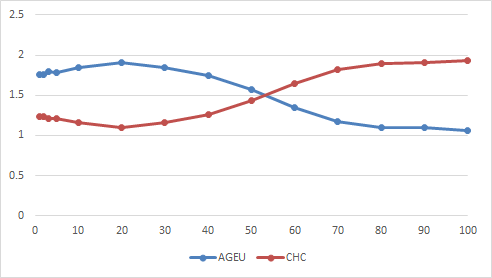
\includegraphics[width=\textwidth]{imagenes/Experimental/AGEUvsCHC.png}
         \caption{Ranking durante todas las \textit{milestones}}
         \label{fig:AGEUvsCHC_lineas}
     \end{subfigure}
     \hfill
     \begin{subfigure}[b]{0.45\textwidth}
         \centering
         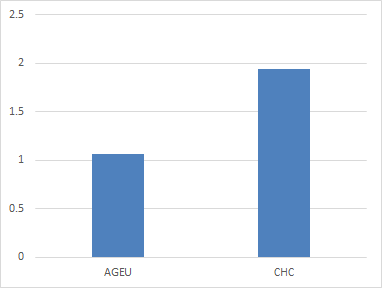
\includegraphics[width=\textwidth]{imagenes/Experimental/barras/AGEUvsCHC.png}
         \caption{Ranking final}
         \label{fig:AGEUvsCHC_barras}
     \end{subfigure}
        \caption{Comparación de AGEU y CHC}
        \label{fig:AGEUvsCHC}
\end{figure}


También podemos apreciar en la tabla \ref{diferenciasAGEU} la media de las distancias entre las soluciones obtenidas en cada \textit{milestone} en la ejecución de AGEU con la final (también más visible en la gráfica \ref{fig:DiferenciasAGEU}). 

%Diferencias AGEU
\begin{table}[]
\begin{tabular}{|cclcclccl|}
\hline
\rowcolor[HTML]{FFFFC7} 
\multicolumn{9}{|c|}{\cellcolor[HTML]{FFFFC7}AGEU   450}                                                                                                                                                                                                                                                                                                                                                                                                                                                                                                 \\ \hline
\rowcolor[HTML]{F7EAC7} 
\multicolumn{1}{|c|}{\cellcolor[HTML]{F7EAC7}n}                               & \multicolumn{1}{c|}{\cellcolor[HTML]{F7EAC7}milestone} & \multicolumn{1}{l|}{\cellcolor[HTML]{F7EAC7}Diferencia} & \multicolumn{1}{c|}{\cellcolor[HTML]{F7EAC7}n}                               & \multicolumn{1}{c|}{\cellcolor[HTML]{F7EAC7}milestone} & \multicolumn{1}{l|}{\cellcolor[HTML]{F7EAC7}Diferencia} & \multicolumn{1}{c|}{\cellcolor[HTML]{F7EAC7}n}                               & \multicolumn{1}{c|}{\cellcolor[HTML]{F7EAC7}milestone} & Diferencia  \\ \hline
\rowcolor[HTML]{DAE8FC} 
\multicolumn{1}{|c|}{\cellcolor[HTML]{FFFFC7}}                                & \multicolumn{1}{c|}{\cellcolor[HTML]{DAE8FC}1}         & \multicolumn{1}{l|}{\cellcolor[HTML]{DAE8FC}20.5989}    & \multicolumn{1}{c|}{\cellcolor[HTML]{FFFFC7}}                                & \multicolumn{1}{c|}{\cellcolor[HTML]{DAE8FC}1}         & \multicolumn{1}{l|}{\cellcolor[HTML]{DAE8FC}27.5017199} & \multicolumn{1}{c|}{\cellcolor[HTML]{FFFFC7}}                                & \multicolumn{1}{c|}{\cellcolor[HTML]{DAE8FC}1}         & 28.8527814  \\ \cline{2-3} \cline{5-6} \cline{8-9} 
\rowcolor[HTML]{DDFDFF} 
\multicolumn{1}{|c|}{\cellcolor[HTML]{FFFFC7}}                                & \multicolumn{1}{c|}{\cellcolor[HTML]{DDFDFF}2}         & \multicolumn{1}{l|}{\cellcolor[HTML]{DDFDFF}16.3468}    & \multicolumn{1}{c|}{\cellcolor[HTML]{FFFFC7}}                                & \multicolumn{1}{c|}{\cellcolor[HTML]{DDFDFF}2}         & \multicolumn{1}{l|}{\cellcolor[HTML]{DDFDFF}22.9143937} & \multicolumn{1}{c|}{\cellcolor[HTML]{FFFFC7}}                                & \multicolumn{1}{c|}{\cellcolor[HTML]{DDFDFF}2}         & 23.90292863 \\ \cline{2-3} \cline{5-6} \cline{8-9} 
\rowcolor[HTML]{DAE8FC} 
\multicolumn{1}{|c|}{\cellcolor[HTML]{FFFFC7}}                                & \multicolumn{1}{c|}{\cellcolor[HTML]{DAE8FC}3}         & \multicolumn{1}{l|}{\cellcolor[HTML]{DAE8FC}14.0108}    & \multicolumn{1}{c|}{\cellcolor[HTML]{FFFFC7}}                                & \multicolumn{1}{c|}{\cellcolor[HTML]{DAE8FC}3}         & \multicolumn{1}{l|}{\cellcolor[HTML]{DAE8FC}20.5848898} & \multicolumn{1}{c|}{\cellcolor[HTML]{FFFFC7}}                                & \multicolumn{1}{c|}{\cellcolor[HTML]{DAE8FC}3}         & 21.25337355 \\ \cline{2-3} \cline{5-6} \cline{8-9} 
\rowcolor[HTML]{DDFDFF} 
\multicolumn{1}{|c|}{\cellcolor[HTML]{FFFFC7}}                                & \multicolumn{1}{c|}{\cellcolor[HTML]{DDFDFF}5}         & \multicolumn{1}{l|}{\cellcolor[HTML]{DDFDFF}10.5074}    & \multicolumn{1}{c|}{\cellcolor[HTML]{FFFFC7}}                                & \multicolumn{1}{c|}{\cellcolor[HTML]{DDFDFF}5}         & \multicolumn{1}{l|}{\cellcolor[HTML]{DDFDFF}16.5204328} & \multicolumn{1}{c|}{\cellcolor[HTML]{FFFFC7}}                                & \multicolumn{1}{c|}{\cellcolor[HTML]{DDFDFF}5}         & 17.2023095  \\ \cline{2-3} \cline{5-6} \cline{8-9} 
\rowcolor[HTML]{DAE8FC} 
\multicolumn{1}{|c|}{\cellcolor[HTML]{FFFFC7}}                                & \multicolumn{1}{c|}{\cellcolor[HTML]{DAE8FC}10}        & \multicolumn{1}{l|}{\cellcolor[HTML]{DAE8FC}5.68841}    & \multicolumn{1}{c|}{\cellcolor[HTML]{FFFFC7}}                                & \multicolumn{1}{c|}{\cellcolor[HTML]{DAE8FC}10}        & \multicolumn{1}{l|}{\cellcolor[HTML]{DAE8FC}10.4844166} & \multicolumn{1}{c|}{\cellcolor[HTML]{FFFFC7}}                                & \multicolumn{1}{c|}{\cellcolor[HTML]{DAE8FC}10}        & 11.26211424 \\ \cline{2-3} \cline{5-6} \cline{8-9} 
\rowcolor[HTML]{DDFDFF} 
\multicolumn{1}{|c|}{\cellcolor[HTML]{FFFFC7}}                                & \multicolumn{1}{c|}{\cellcolor[HTML]{DDFDFF}20}        & \multicolumn{1}{l|}{\cellcolor[HTML]{DDFDFF}2.33124}    & \multicolumn{1}{c|}{\cellcolor[HTML]{FFFFC7}}                                & \multicolumn{1}{c|}{\cellcolor[HTML]{DDFDFF}20}        & \multicolumn{1}{l|}{\cellcolor[HTML]{DDFDFF}5.40382962} & \multicolumn{1}{c|}{\cellcolor[HTML]{FFFFC7}}                                & \multicolumn{1}{c|}{\cellcolor[HTML]{DDFDFF}20}        & 6.370632961 \\ \cline{2-3} \cline{5-6} \cline{8-9} 
\rowcolor[HTML]{DAE8FC} 
\multicolumn{1}{|c|}{\cellcolor[HTML]{FFFFC7}}                                & \multicolumn{1}{c|}{\cellcolor[HTML]{DAE8FC}30}        & \multicolumn{1}{l|}{\cellcolor[HTML]{DAE8FC}1.1489}     & \multicolumn{1}{c|}{\cellcolor[HTML]{FFFFC7}}                                & \multicolumn{1}{c|}{\cellcolor[HTML]{DAE8FC}30}        & \multicolumn{1}{l|}{\cellcolor[HTML]{DAE8FC}3.14660193} & \multicolumn{1}{c|}{\cellcolor[HTML]{FFFFC7}}                                & \multicolumn{1}{c|}{\cellcolor[HTML]{DAE8FC}30}        & 4.193702678 \\ \cline{2-3} \cline{5-6} \cline{8-9} 
\rowcolor[HTML]{DDFDFF} 
\multicolumn{1}{|c|}{\cellcolor[HTML]{FFFFC7}}                                & \multicolumn{1}{c|}{\cellcolor[HTML]{DDFDFF}40}        & \multicolumn{1}{l|}{\cellcolor[HTML]{DDFDFF}0.6321}     & \multicolumn{1}{c|}{\cellcolor[HTML]{FFFFC7}}                                & \multicolumn{1}{c|}{\cellcolor[HTML]{DDFDFF}40}        & \multicolumn{1}{l|}{\cellcolor[HTML]{DDFDFF}1.87304152} & \multicolumn{1}{c|}{\cellcolor[HTML]{FFFFC7}}                                & \multicolumn{1}{c|}{\cellcolor[HTML]{DDFDFF}40}        & 2.913529408 \\ \cline{2-3} \cline{5-6} \cline{8-9} 
\rowcolor[HTML]{DAE8FC} 
\multicolumn{1}{|c|}{\cellcolor[HTML]{FFFFC7}}                                & \multicolumn{1}{c|}{\cellcolor[HTML]{DAE8FC}50}        & \multicolumn{1}{l|}{\cellcolor[HTML]{DAE8FC}0.36445}    & \multicolumn{1}{c|}{\cellcolor[HTML]{FFFFC7}}                                & \multicolumn{1}{c|}{\cellcolor[HTML]{DAE8FC}50}        & \multicolumn{1}{l|}{\cellcolor[HTML]{DAE8FC}1.10940335} & \multicolumn{1}{c|}{\cellcolor[HTML]{FFFFC7}}                                & \multicolumn{1}{c|}{\cellcolor[HTML]{DAE8FC}50}        & 1.986383412 \\ \cline{2-3} \cline{5-6} \cline{8-9} 
\rowcolor[HTML]{DDFDFF} 
\multicolumn{1}{|c|}{\cellcolor[HTML]{FFFFC7}}                                & \multicolumn{1}{c|}{\cellcolor[HTML]{DDFDFF}60}        & \multicolumn{1}{l|}{\cellcolor[HTML]{DDFDFF}0.20967}    & \multicolumn{1}{c|}{\cellcolor[HTML]{FFFFC7}}                                & \multicolumn{1}{c|}{\cellcolor[HTML]{DDFDFF}60}        & \multicolumn{1}{l|}{\cellcolor[HTML]{DDFDFF}0.64701591} & \multicolumn{1}{c|}{\cellcolor[HTML]{FFFFC7}}                                & \multicolumn{1}{c|}{\cellcolor[HTML]{DDFDFF}60}        & 1.330223249 \\ \cline{2-3} \cline{5-6} \cline{8-9} 
\rowcolor[HTML]{DAE8FC} 
\multicolumn{1}{|c|}{\cellcolor[HTML]{FFFFC7}}                                & \multicolumn{1}{c|}{\cellcolor[HTML]{DAE8FC}70}        & \multicolumn{1}{l|}{\cellcolor[HTML]{DAE8FC}0.12326}    & \multicolumn{1}{c|}{\cellcolor[HTML]{FFFFC7}}                                & \multicolumn{1}{c|}{\cellcolor[HTML]{DAE8FC}70}        & \multicolumn{1}{l|}{\cellcolor[HTML]{DAE8FC}0.3791851}  & \multicolumn{1}{c|}{\cellcolor[HTML]{FFFFC7}}                                & \multicolumn{1}{c|}{\cellcolor[HTML]{DAE8FC}70}        & 0.852926436 \\ \cline{2-3} \cline{5-6} \cline{8-9} 
\rowcolor[HTML]{DDFDFF} 
\multicolumn{1}{|c|}{\cellcolor[HTML]{FFFFC7}}                                & \multicolumn{1}{c|}{\cellcolor[HTML]{DDFDFF}80}        & \multicolumn{1}{l|}{\cellcolor[HTML]{DDFDFF}0.07038}    & \multicolumn{1}{c|}{\cellcolor[HTML]{FFFFC7}}                                & \multicolumn{1}{c|}{\cellcolor[HTML]{DDFDFF}80}        & \multicolumn{1}{l|}{\cellcolor[HTML]{DDFDFF}0.20608454} & \multicolumn{1}{c|}{\cellcolor[HTML]{FFFFC7}}                                & \multicolumn{1}{c|}{\cellcolor[HTML]{DDFDFF}80}        & 0.475363912 \\ \cline{2-3} \cline{5-6} \cline{8-9} 
\rowcolor[HTML]{DAE8FC} 
\multicolumn{1}{|c|}{\multirow{-13}{*}{\cellcolor[HTML]{FFFFC7}\textbf{100}}} & \multicolumn{1}{c|}{\cellcolor[HTML]{DAE8FC}90}        & \multicolumn{1}{l|}{\cellcolor[HTML]{DAE8FC}0.03592}    & \multicolumn{1}{c|}{\multirow{-13}{*}{\cellcolor[HTML]{FFFFC7}\textbf{200}}} & \multicolumn{1}{c|}{\cellcolor[HTML]{DAE8FC}90}        & \multicolumn{1}{l|}{\cellcolor[HTML]{DAE8FC}0.08155519} & \multicolumn{1}{c|}{\multirow{-13}{*}{\cellcolor[HTML]{FFFFC7}\textbf{300}}} & \multicolumn{1}{c|}{\cellcolor[HTML]{DAE8FC}90}        & 0.198954275 \\ \hline
\end{tabular}
\caption{\label{diferenciasAGEU}Diferencias de los resultados de las distintas milestones con respecto a la final para el AG}
\end{table}

\begin{figure}
		\centering
		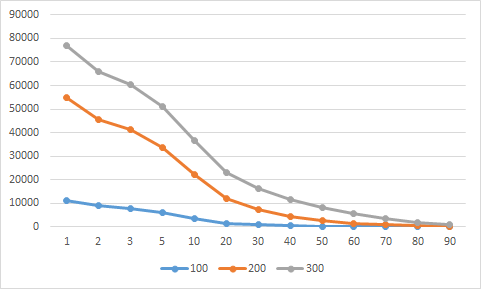
\includegraphics[scale=1]{imagenes/Experimental/DiferenciasAGEU.png}
        \caption{Gráfica asociada a la tabla \ref{diferenciasAGEU}}
        \label{fig:DiferenciasAGEU}
\end{figure}

De la misma forma, en la tabla \ref{DiferenciasCHC} se puede apreciar la media de las diferencias entre las soluciones obtenidas en cada \textit{milestone} de la ejecución del algoritmo CHC con la final (también más visible en la gráfica \ref{fig:DiferenciasCHC}). 

%Diferencias CHC
\begin{table}[]
\begin{tabular}{|cclcclccl|}
\hline
\rowcolor[HTML]{FFFFC7} 
\multicolumn{9}{|c|}{\cellcolor[HTML]{FFFFC7}CHC   450}                                                                                                                                                                                                                                                                                                                                                                                                                                                                                                 \\ \hline
\rowcolor[HTML]{F7EAC7} 
\multicolumn{1}{|c|}{\cellcolor[HTML]{F7EAC7}n}                               & \multicolumn{1}{c|}{\cellcolor[HTML]{F7EAC7}milestone} & \multicolumn{1}{l|}{\cellcolor[HTML]{F7EAC7}Diferencia} & \multicolumn{1}{c|}{\cellcolor[HTML]{F7EAC7}n}                               & \multicolumn{1}{c|}{\cellcolor[HTML]{F7EAC7}milestone} & \multicolumn{1}{l|}{\cellcolor[HTML]{F7EAC7}Diferencia} & \multicolumn{1}{c|}{\cellcolor[HTML]{F7EAC7}n}                               & \multicolumn{1}{c|}{\cellcolor[HTML]{F7EAC7}milestone} & Diferencia \\ \hline
\rowcolor[HTML]{DAE8FC} 
\multicolumn{1}{|c|}{\cellcolor[HTML]{FFFFC7}}                                & \multicolumn{1}{c|}{\cellcolor[HTML]{DAE8FC}1}         & \multicolumn{1}{l|}{\cellcolor[HTML]{DAE8FC}12.8016}    & \multicolumn{1}{c|}{\cellcolor[HTML]{FFFFC7}}                                & \multicolumn{1}{c|}{\cellcolor[HTML]{DAE8FC}1}         & \multicolumn{1}{l|}{\cellcolor[HTML]{DAE8FC}19.8850218} & \multicolumn{1}{c|}{\cellcolor[HTML]{FFFFC7}}                                & \multicolumn{1}{c|}{\cellcolor[HTML]{DAE8FC}1}         & 31.0012675 \\ \cline{2-3} \cline{5-6} \cline{8-9} 
\rowcolor[HTML]{DDFDFF} 
\multicolumn{1}{|c|}{\cellcolor[HTML]{FFFFC7}}                                & \multicolumn{1}{c|}{\cellcolor[HTML]{DDFDFF}2}         & \multicolumn{1}{l|}{\cellcolor[HTML]{DDFDFF}9.87116}    & \multicolumn{1}{c|}{\cellcolor[HTML]{FFFFC7}}                                & \multicolumn{1}{c|}{\cellcolor[HTML]{DDFDFF}2}         & \multicolumn{1}{l|}{\cellcolor[HTML]{DDFDFF}17.2722142} & \multicolumn{1}{c|}{\cellcolor[HTML]{FFFFC7}}                                & \multicolumn{1}{c|}{\cellcolor[HTML]{DDFDFF}2}         & 29.0482187 \\ \cline{2-3} \cline{5-6} \cline{8-9} 
\rowcolor[HTML]{DAE8FC} 
\multicolumn{1}{|c|}{\cellcolor[HTML]{FFFFC7}}                                & \multicolumn{1}{c|}{\cellcolor[HTML]{DAE8FC}3}         & \multicolumn{1}{l|}{\cellcolor[HTML]{DAE8FC}7.03101}    & \multicolumn{1}{c|}{\cellcolor[HTML]{FFFFC7}}                                & \multicolumn{1}{c|}{\cellcolor[HTML]{DAE8FC}3}         & \multicolumn{1}{l|}{\cellcolor[HTML]{DAE8FC}15.6907262} & \multicolumn{1}{c|}{\cellcolor[HTML]{FFFFC7}}                                & \multicolumn{1}{c|}{\cellcolor[HTML]{DAE8FC}3}         & 27.939129  \\ \cline{2-3} \cline{5-6} \cline{8-9} 
\rowcolor[HTML]{DDFDFF} 
\multicolumn{1}{|c|}{\cellcolor[HTML]{FFFFC7}}                                & \multicolumn{1}{c|}{\cellcolor[HTML]{DDFDFF}5}         & \multicolumn{1}{l|}{\cellcolor[HTML]{DDFDFF}4.13105}    & \multicolumn{1}{c|}{\cellcolor[HTML]{FFFFC7}}                                & \multicolumn{1}{c|}{\cellcolor[HTML]{DDFDFF}5}         & \multicolumn{1}{l|}{\cellcolor[HTML]{DDFDFF}13.1825268} & \multicolumn{1}{c|}{\cellcolor[HTML]{FFFFC7}}                                & \multicolumn{1}{c|}{\cellcolor[HTML]{DDFDFF}5}         & 25.9419819 \\ \cline{2-3} \cline{5-6} \cline{8-9} 
\rowcolor[HTML]{DAE8FC} 
\multicolumn{1}{|c|}{\cellcolor[HTML]{FFFFC7}}                                & \multicolumn{1}{c|}{\cellcolor[HTML]{DAE8FC}10}        & \multicolumn{1}{l|}{\cellcolor[HTML]{DAE8FC}0.66658}    & \multicolumn{1}{c|}{\cellcolor[HTML]{FFFFC7}}                                & \multicolumn{1}{c|}{\cellcolor[HTML]{DAE8FC}10}        & \multicolumn{1}{l|}{\cellcolor[HTML]{DAE8FC}5.55650253} & \multicolumn{1}{c|}{\cellcolor[HTML]{FFFFC7}}                                & \multicolumn{1}{c|}{\cellcolor[HTML]{DAE8FC}10}        & 18.8008051 \\ \cline{2-3} \cline{5-6} \cline{8-9} 
\rowcolor[HTML]{DDFDFF} 
\multicolumn{1}{|c|}{\cellcolor[HTML]{FFFFC7}}                                & \multicolumn{1}{c|}{\cellcolor[HTML]{DDFDFF}20}        & \multicolumn{1}{l|}{\cellcolor[HTML]{DDFDFF}0.00171}    & \multicolumn{1}{c|}{\cellcolor[HTML]{FFFFC7}}                                & \multicolumn{1}{c|}{\cellcolor[HTML]{DDFDFF}20}        & \multicolumn{1}{l|}{\cellcolor[HTML]{DDFDFF}0.36295397} & \multicolumn{1}{c|}{\cellcolor[HTML]{FFFFC7}}                                & \multicolumn{1}{c|}{\cellcolor[HTML]{DDFDFF}20}        & 2.2348952  \\ \cline{2-3} \cline{5-6} \cline{8-9} 
\rowcolor[HTML]{DAE8FC} 
\multicolumn{1}{|c|}{\cellcolor[HTML]{FFFFC7}}                                & \multicolumn{1}{c|}{\cellcolor[HTML]{DAE8FC}30}        & \multicolumn{1}{l|}{\cellcolor[HTML]{DAE8FC}2.5E-05}    & \multicolumn{1}{c|}{\cellcolor[HTML]{FFFFC7}}                                & \multicolumn{1}{c|}{\cellcolor[HTML]{DAE8FC}30}        & \multicolumn{1}{l|}{\cellcolor[HTML]{DAE8FC}0.00250816} & \multicolumn{1}{c|}{\cellcolor[HTML]{FFFFC7}}                                & \multicolumn{1}{c|}{\cellcolor[HTML]{DAE8FC}30}        & 0.15429962 \\ \cline{2-3} \cline{5-6} \cline{8-9} 
\rowcolor[HTML]{DDFDFF} 
\multicolumn{1}{|c|}{\cellcolor[HTML]{FFFFC7}}                                & \multicolumn{1}{c|}{\cellcolor[HTML]{DDFDFF}40}        & \multicolumn{1}{l|}{\cellcolor[HTML]{DDFDFF}0}          & \multicolumn{1}{c|}{\cellcolor[HTML]{FFFFC7}}                                & \multicolumn{1}{c|}{\cellcolor[HTML]{DDFDFF}40}        & \multicolumn{1}{l|}{\cellcolor[HTML]{DDFDFF}0.00030503} & \multicolumn{1}{c|}{\cellcolor[HTML]{FFFFC7}}                                & \multicolumn{1}{c|}{\cellcolor[HTML]{DDFDFF}40}        & 0.00179232 \\ \cline{2-3} \cline{5-6} \cline{8-9} 
\rowcolor[HTML]{DAE8FC} 
\multicolumn{1}{|c|}{\cellcolor[HTML]{FFFFC7}}                                & \multicolumn{1}{c|}{\cellcolor[HTML]{DAE8FC}50}        & \multicolumn{1}{l|}{\cellcolor[HTML]{DAE8FC}0}          & \multicolumn{1}{c|}{\cellcolor[HTML]{FFFFC7}}                                & \multicolumn{1}{c|}{\cellcolor[HTML]{DAE8FC}50}        & \multicolumn{1}{l|}{\cellcolor[HTML]{DAE8FC}6.9674E-05} & \multicolumn{1}{c|}{\cellcolor[HTML]{FFFFC7}}                                & \multicolumn{1}{c|}{\cellcolor[HTML]{DAE8FC}50}        & 7.5388E-05 \\ \cline{2-3} \cline{5-6} \cline{8-9} 
\rowcolor[HTML]{DDFDFF} 
\multicolumn{1}{|c|}{\cellcolor[HTML]{FFFFC7}}                                & \multicolumn{1}{c|}{\cellcolor[HTML]{DDFDFF}60}        & \multicolumn{1}{l|}{\cellcolor[HTML]{DDFDFF}0}          & \multicolumn{1}{c|}{\cellcolor[HTML]{FFFFC7}}                                & \multicolumn{1}{c|}{\cellcolor[HTML]{DDFDFF}60}        & \multicolumn{1}{l|}{\cellcolor[HTML]{DDFDFF}0}          & \multicolumn{1}{c|}{\cellcolor[HTML]{FFFFC7}}                                & \multicolumn{1}{c|}{\cellcolor[HTML]{DDFDFF}60}        & 0          \\ \cline{2-3} \cline{5-6} \cline{8-9} 
\rowcolor[HTML]{DAE8FC} 
\multicolumn{1}{|c|}{\cellcolor[HTML]{FFFFC7}}                                & \multicolumn{1}{c|}{\cellcolor[HTML]{DAE8FC}70}        & \multicolumn{1}{l|}{\cellcolor[HTML]{DAE8FC}0}          & \multicolumn{1}{c|}{\cellcolor[HTML]{FFFFC7}}                                & \multicolumn{1}{c|}{\cellcolor[HTML]{DAE8FC}70}        & \multicolumn{1}{l|}{\cellcolor[HTML]{DAE8FC}0}          & \multicolumn{1}{c|}{\cellcolor[HTML]{FFFFC7}}                                & \multicolumn{1}{c|}{\cellcolor[HTML]{DAE8FC}70}        & 0          \\ \cline{2-3} \cline{5-6} \cline{8-9} 
\rowcolor[HTML]{DDFDFF} 
\multicolumn{1}{|c|}{\cellcolor[HTML]{FFFFC7}}                                & \multicolumn{1}{c|}{\cellcolor[HTML]{DDFDFF}80}        & \multicolumn{1}{l|}{\cellcolor[HTML]{DDFDFF}0}          & \multicolumn{1}{c|}{\cellcolor[HTML]{FFFFC7}}                                & \multicolumn{1}{c|}{\cellcolor[HTML]{DDFDFF}80}        & \multicolumn{1}{l|}{\cellcolor[HTML]{DDFDFF}0}          & \multicolumn{1}{c|}{\cellcolor[HTML]{FFFFC7}}                                & \multicolumn{1}{c|}{\cellcolor[HTML]{DDFDFF}80}        & 0          \\ \cline{2-3} \cline{5-6} \cline{8-9} 
\rowcolor[HTML]{DAE8FC} 
\multicolumn{1}{|c|}{\multirow{-13}{*}{\cellcolor[HTML]{FFFFC7}\textbf{100}}} & \multicolumn{1}{c|}{\cellcolor[HTML]{DAE8FC}90}        & \multicolumn{1}{l|}{\cellcolor[HTML]{DAE8FC}0}          & \multicolumn{1}{c|}{\multirow{-13}{*}{\cellcolor[HTML]{FFFFC7}\textbf{200}}} & \multicolumn{1}{c|}{\cellcolor[HTML]{DAE8FC}90}        & \multicolumn{1}{l|}{\cellcolor[HTML]{DAE8FC}0}          & \multicolumn{1}{c|}{\multirow{-13}{*}{\cellcolor[HTML]{FFFFC7}\textbf{300}}} & \multicolumn{1}{c|}{\cellcolor[HTML]{DAE8FC}90}        & 0          \\ \hline
\end{tabular}
\caption{\label{DiferenciasCHC}Diferencias de los resultados de las distintas milestones con respecto a la final para el algoritmo CHC}
\end{table}

\begin{figure}[h]
		\centering
		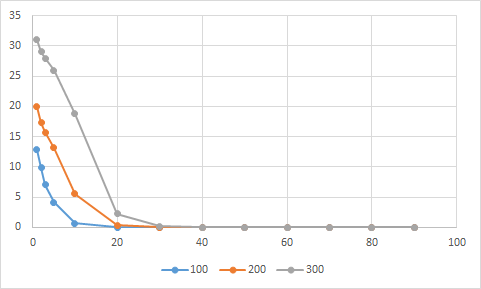
\includegraphics[scale=1]{imagenes/Experimental/DiferenciasCHC.png}
        \caption{Gráfica asociada a la tabla \ref{DiferenciasCHC}}
        \label{fig:DiferenciasCHC}
\end{figure}

Por lo que se puede ver en la tabla \ref{diferenciasAGEU} no se puede decir que converja prematuramente, de hecho en todo momento realiza mejoras significativas. 
Esto se puede observar en el hecho de que las diferencias a la última solución van disminuyendo en gran medida en cada una de las \textit{milestones}. 

Sin embargo, en la tabla \ref{DiferenciasCHC} se tiene que las soluciones convergen rápidamente a la solución final antes de llegar siquiera el 50\% de la ejecución total. 
De esto se puede inferir que los mecanismos de aumento de la diversidad de CHC no son de mucha utilidad en nuestro caso. 
También se debe tener en cuenta que estamos usando una modificación de CHC donde no se reinicia la población, ya que se prevee su rápida convergencia, lo que causaría una gran cantidad de reinicios y, por tanto, evaluaciones, las cuales estamos intentando mantener al mínimo. 
En contrapartida a no usar reinicio de población, se mantiene la mutación de las soluciones con el fin de aportar más diversidad. 
A vista de los resultados se puede entender que esto no es suficiente para mantener la diversidad. 

Por otra parte, si nos fijamos en la gráfica \ref{fig:AGEUvsCHC} se puede ver cómo el algoritmo CHC es mejor que el AGEU mientras que se siguen produciendo cambios, es decir, antes de que se produzca el 50\% de la ejecución. 
Por lo que se considerará posteriormente una mezcla de ambos algoritmos, con el fin de aprovechar los buenos resultados iniciales del CHC y la capacidad de no converger rápidamente que presenta AGEU con el fin de tener un buen punto de partida.

\section{Incorporación del histórico}

La primera modificación que se propone es la introducción de un histórico \ref{alg:Historico_Estructura}, explicado en la primera sección del capítulo anterior. 
La principal motivación de esta modificación es incidir en la explotación de las buenas soluciones, ya que se almacenarán los elementos más predominantes en las mejores soluciones y en las peores, con el fin de reincidir con mayor frecuencia en los primeros y rehuir de los segundos. 

Obviamente, este histórico deberá tener un proceso de aprendizaje (en el que almacena todas las soluciones distintas para luego discernir cuáles son las mejores y cuáles las peores y sus respectivos elementos) y un proceso de reacción, en la que pondrá en práctica la información aprendida en la fase anterior. 
Con el fin de que no sea un único procedimiento y pueda ir aprendiendo a lo largo de la ejecución (para intentar evitar quedarse en máximos locales), estas dos fases se irán turnando cada 50 generaciones. 

Para poner a prueba su utilidad, se estudian los resultados obtenidos de aplicar el histórico solo al operador de reparación (si tiene que añadir elementos, elegirá los mejores; si tiene que eliminar elementos, elegirá los peores), solo a la mutación (tiene prioridad insertar mejores elementos y eliminar peores) y a ambos a la vez. 
Los resultados de este estudio se muestran en la tablas \ref{HistMut}, \ref{HistCruce} y \ref{GACEPv1} y, más visualmente, en la gráfica \ref{fig:Historico}.

\begin{figure}
     \centering
     \begin{subfigure}[b]{0.45\textwidth}
         \centering
         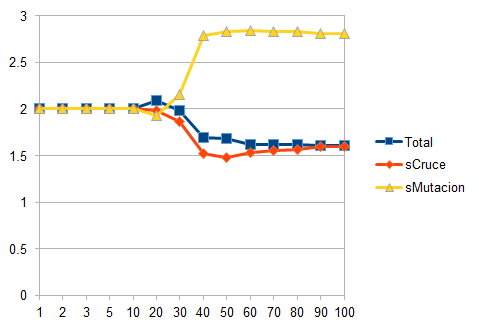
\includegraphics[width=\textwidth]{imagenes/Experimental/Historico.png}
         \caption{Ranking durante todas las \textit{milestones}}
         \label{fig:Historico_lineas}
     \end{subfigure}
     \hfill
     \begin{subfigure}[b]{0.45\textwidth}
         \centering
         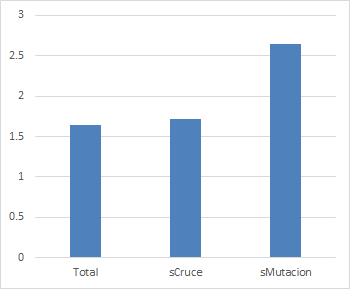
\includegraphics[width=\textwidth]{imagenes/Experimental/barras/Historico.png}
         \caption{Ranking final}
         \label{fig:Historico_barras}
     \end{subfigure}
        \caption{Comparación de las distintas versiones del histórico}
        \label{fig:Historico}
\end{figure}

En esta gráfica \ref{fig:Historico} podemos apreciar que las mejores opciones son aplicarlo solo al cruce o a ambos; de hecho, por muy poco se tiene que aplicar ambas modificaciones es lo mejor. 
El uso de ambas opciones también viene justificado por un intento de mantener la consistencia, y porque es posible que en algún momento del desarrollo se puedan realizar más modificaciones a la mutación de las que el histórico se podría aprovechar. 

Además, que cuando solo se aplique el histórico a la mutación de los peores resultados con diferencia es una primera indicación de que la introducción del histórico ha supuesto una mejora al modelo original.
Esto se debe a que realmente la mutación se produce un número muy bajo de veces y no suele producir grandes cambios, por lo que si es lo único que se modifica, es muy probable que no se distancie mucho de los resultados originales. 
Para confirmar esta idea y poder asegurarnos de que se ha dado un paso en una dirección correcta, comparamos en la gráfica \ref{fig:AGEUvsGACEPv1} los resultados originales y los de aplicar el histórico a ambos operadores. 

\begin{figure}
     \centering
     \begin{subfigure}[b]{0.45\textwidth}
         \centering
         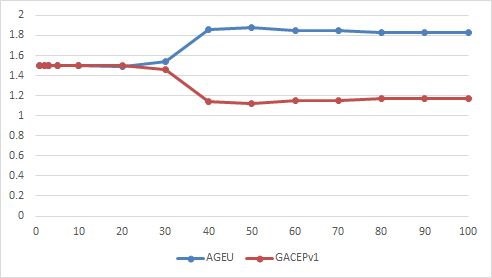
\includegraphics[width=\textwidth]{imagenes/Experimental/AGEUvsGACEPv1.png}
         \caption{Ranking durante todas las \textit{milestones}}
         \label{fig:AGEUvsGACEPv1_lineas}
     \end{subfigure}
     \hfill
     \begin{subfigure}[b]{0.45\textwidth}
         \centering
         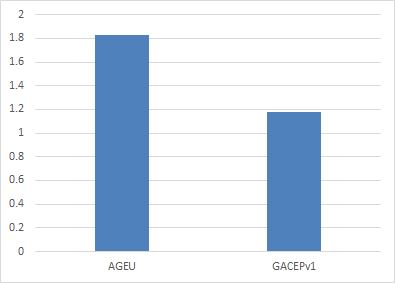
\includegraphics[width=\textwidth]{imagenes/Experimental/barras/AGEUvsGACEPv1.png}
         \caption{Ranking final}
         \label{fig:AGEUvsGACEPv1_barras}
     \end{subfigure}
        \caption{Comparación de los resultados del AGEU y GACEPv1}
        \label{fig:AGEUvsGACEPv1}
\end{figure}

Con esta gráfica \ref{fig:AGEUvsGACEPv1} quedan confirmadas nuestras suposiciones. 
Es importante mencionar que en sus primeras iteraciones ambos algoritmos obtienen los mismos resultados ya que se comportan de la misma forma. 
Recordemos que cada fase del histórico ocupa 50 iteraciones, por lo que durante las primeras 50 iteraciones va a mantener el mismo comportamiento que AGEU, con la excepción de que va a ir almacenando las soluciones para su posterior análisis. 
Estas 50 iteraciones suponen un poco más del 10\% inicial de las iteraciones totales, por lo que es obvio que para todas estas \textit{milestones} sus resultados van a ser iguales. 
También cabe la pena mencionar que en el momento en el que difieren los resultados de los algoritmos, su clasificación se mantiene casi constante, por lo que queda claro que el uso del histórico hace que el algoritmo sea consistentemente mejor.  

Es más, con esta modificación podemos crear las bases de lo que será nuestro nuevo algoritmo, al cual llamaremos \textbf{GACEP} (\textbf{\textit{Genetic Algorithm for Combinatory Expensive Problem}}). 
Para establecer una notación común entre las distintas modificaciones, todas se nombrarán de la forma ``GACEPv\texttt{x}'', donde \texttt{x} se sustituirá por el número de la versión. 
En este caso, el introducir el histórico al AG lo llamaremos \textbf{GACEPv1}.

Los resultados de la ejecución de este algoritmo vienen recopilados en la tabla \ref{GACEPv1}.

A continuación haremos lo mismo que para los algoritmos de referencia y observaremos si se ha producido algún tipo de convergencia prematura. 
Esto se puede ver en la tabla \ref{DiferenciasGACEPv1} y en su gráfica asociada \ref{fig:DiferenciasGACEPv1}.

%Diferencias GACEP
\begin{table}[]
\begin{tabular}{|cclcclccl|}
\hline
\rowcolor[HTML]{FFFFC7} 
\multicolumn{9}{|c|}{\cellcolor[HTML]{FFFFC7}GACEPv1}                                                                                                                                                                                                                                                                                                                                                                                                                                                                        \\ \hline
\rowcolor[HTML]{F7EAC7} 
\multicolumn{1}{|c|}{\cellcolor[HTML]{F7EAC7}n}                      & \multicolumn{1}{c|}{\cellcolor[HTML]{F7EAC7}milestone} & \multicolumn{1}{l|}{\cellcolor[HTML]{F7EAC7}Diferencia} & \multicolumn{1}{c|}{\cellcolor[HTML]{F7EAC7}n}                      & \multicolumn{1}{c|}{\cellcolor[HTML]{F7EAC7}milestone} & \multicolumn{1}{l|}{\cellcolor[HTML]{F7EAC7}Diferencia} & \multicolumn{1}{c|}{\cellcolor[HTML]{F7EAC7}n}                      & \multicolumn{1}{c|}{\cellcolor[HTML]{F7EAC7}milestone} & Diferencia \\ \hline
\rowcolor[HTML]{DAE8FC} 
\multicolumn{1}{|c|}{\cellcolor[HTML]{FFFFC7}}                       & \multicolumn{1}{c|}{\cellcolor[HTML]{DAE8FC}1}         & \multicolumn{1}{l|}{\cellcolor[HTML]{DAE8FC}24.8702}    & \multicolumn{1}{c|}{\cellcolor[HTML]{FFFFC7}}                       & \multicolumn{1}{c|}{\cellcolor[HTML]{DAE8FC}1}         & \multicolumn{1}{l|}{\cellcolor[HTML]{DAE8FC}28.9265669} & \multicolumn{1}{c|}{\cellcolor[HTML]{FFFFC7}}                       & \multicolumn{1}{c|}{\cellcolor[HTML]{DAE8FC}1}         & 28.4705381 \\ \cline{2-3} \cline{5-6} \cline{8-9} 
\rowcolor[HTML]{DDFDFF} 
\multicolumn{1}{|c|}{\cellcolor[HTML]{FFFFC7}}                       & \multicolumn{1}{c|}{\cellcolor[HTML]{DDFDFF}2}         & \multicolumn{1}{l|}{\cellcolor[HTML]{DDFDFF}20.8839}    & \multicolumn{1}{c|}{\cellcolor[HTML]{FFFFC7}}                       & \multicolumn{1}{c|}{\cellcolor[HTML]{DDFDFF}2}         & \multicolumn{1}{l|}{\cellcolor[HTML]{DDFDFF}24.473429}  & \multicolumn{1}{c|}{\cellcolor[HTML]{FFFFC7}}                       & \multicolumn{1}{c|}{\cellcolor[HTML]{DDFDFF}2}         & 23.6064829 \\ \cline{2-3} \cline{5-6} \cline{8-9} 
\rowcolor[HTML]{DAE8FC} 
\multicolumn{1}{|c|}{\cellcolor[HTML]{FFFFC7}}                       & \multicolumn{1}{c|}{\cellcolor[HTML]{DAE8FC}3}         & \multicolumn{1}{l|}{\cellcolor[HTML]{DAE8FC}18.6934}    & \multicolumn{1}{c|}{\cellcolor[HTML]{FFFFC7}}                       & \multicolumn{1}{c|}{\cellcolor[HTML]{DAE8FC}3}         & \multicolumn{1}{l|}{\cellcolor[HTML]{DAE8FC}22.2164778} & \multicolumn{1}{c|}{\cellcolor[HTML]{FFFFC7}}                       & \multicolumn{1}{c|}{\cellcolor[HTML]{DAE8FC}3}         & 21.0057888 \\ \cline{2-3} \cline{5-6} \cline{8-9} 
\rowcolor[HTML]{DDFDFF} 
\multicolumn{1}{|c|}{\cellcolor[HTML]{FFFFC7}}                       & \multicolumn{1}{c|}{\cellcolor[HTML]{DDFDFF}5}         & \multicolumn{1}{l|}{\cellcolor[HTML]{DDFDFF}15.4131}    & \multicolumn{1}{c|}{\cellcolor[HTML]{FFFFC7}}                       & \multicolumn{1}{c|}{\cellcolor[HTML]{DDFDFF}5}         & \multicolumn{1}{l|}{\cellcolor[HTML]{DDFDFF}18.2724015} & \multicolumn{1}{c|}{\cellcolor[HTML]{FFFFC7}}                       & \multicolumn{1}{c|}{\cellcolor[HTML]{DDFDFF}5}         & 17.0150669 \\ \cline{2-3} \cline{5-6} \cline{8-9} 
\rowcolor[HTML]{DAE8FC} 
\multicolumn{1}{|c|}{\cellcolor[HTML]{FFFFC7}}                       & \multicolumn{1}{c|}{\cellcolor[HTML]{DAE8FC}10}        & \multicolumn{1}{l|}{\cellcolor[HTML]{DAE8FC}10.9019}    & \multicolumn{1}{c|}{\cellcolor[HTML]{FFFFC7}}                       & \multicolumn{1}{c|}{\cellcolor[HTML]{DAE8FC}10}        & \multicolumn{1}{l|}{\cellcolor[HTML]{DAE8FC}12.4140872} & \multicolumn{1}{c|}{\cellcolor[HTML]{FFFFC7}}                       & \multicolumn{1}{c|}{\cellcolor[HTML]{DAE8FC}10}        & 11.1442233 \\ \cline{2-3} \cline{5-6} \cline{8-9} 
\rowcolor[HTML]{DDFDFF} 
\multicolumn{1}{|c|}{\cellcolor[HTML]{FFFFC7}}                       & \multicolumn{1}{c|}{\cellcolor[HTML]{DDFDFF}20}        & \multicolumn{1}{l|}{\cellcolor[HTML]{DDFDFF}5.64471}    & \multicolumn{1}{c|}{\cellcolor[HTML]{FFFFC7}}                       & \multicolumn{1}{c|}{\cellcolor[HTML]{DDFDFF}20}        & \multicolumn{1}{l|}{\cellcolor[HTML]{DDFDFF}8.14923733} & \multicolumn{1}{c|}{\cellcolor[HTML]{FFFFC7}}                       & \multicolumn{1}{c|}{\cellcolor[HTML]{DDFDFF}20}        & 6.84098075 \\ \cline{2-3} \cline{5-6} \cline{8-9} 
\rowcolor[HTML]{DAE8FC} 
\multicolumn{1}{|c|}{\cellcolor[HTML]{FFFFC7}}                       & \multicolumn{1}{c|}{\cellcolor[HTML]{DAE8FC}30}        & \multicolumn{1}{l|}{\cellcolor[HTML]{DAE8FC}4.10969}    & \multicolumn{1}{c|}{\cellcolor[HTML]{FFFFC7}}                       & \multicolumn{1}{c|}{\cellcolor[HTML]{DAE8FC}30}        & \multicolumn{1}{l|}{\cellcolor[HTML]{DAE8FC}5.35892582} & \multicolumn{1}{c|}{\cellcolor[HTML]{FFFFC7}}                       & \multicolumn{1}{c|}{\cellcolor[HTML]{DAE8FC}30}        & 4.4650068  \\ \cline{2-3} \cline{5-6} \cline{8-9} 
\rowcolor[HTML]{DDFDFF} 
\multicolumn{1}{|c|}{\cellcolor[HTML]{FFFFC7}}                       & \multicolumn{1}{c|}{\cellcolor[HTML]{DDFDFF}40}        & \multicolumn{1}{l|}{\cellcolor[HTML]{DDFDFF}1.43438}    & \multicolumn{1}{c|}{\cellcolor[HTML]{FFFFC7}}                       & \multicolumn{1}{c|}{\cellcolor[HTML]{DDFDFF}40}        & \multicolumn{1}{l|}{\cellcolor[HTML]{DDFDFF}2.30317627} & \multicolumn{1}{c|}{\cellcolor[HTML]{FFFFC7}}                       & \multicolumn{1}{c|}{\cellcolor[HTML]{DDFDFF}40}        & 2.05939817 \\ \cline{2-3} \cline{5-6} \cline{8-9} 
\rowcolor[HTML]{DAE8FC} 
\multicolumn{1}{|c|}{\cellcolor[HTML]{FFFFC7}}                       & \multicolumn{1}{c|}{\cellcolor[HTML]{DAE8FC}50}        & \multicolumn{1}{l|}{\cellcolor[HTML]{DAE8FC}0.63711}    & \multicolumn{1}{c|}{\cellcolor[HTML]{FFFFC7}}                       & \multicolumn{1}{c|}{\cellcolor[HTML]{DAE8FC}50}        & \multicolumn{1}{l|}{\cellcolor[HTML]{DAE8FC}0.97838195} & \multicolumn{1}{c|}{\cellcolor[HTML]{FFFFC7}}                       & \multicolumn{1}{c|}{\cellcolor[HTML]{DAE8FC}50}        & 1.03637898 \\ \cline{2-3} \cline{5-6} \cline{8-9} 
\rowcolor[HTML]{DDFDFF} 
\multicolumn{1}{|c|}{\cellcolor[HTML]{FFFFC7}}                       & \multicolumn{1}{c|}{\cellcolor[HTML]{DDFDFF}60}        & \multicolumn{1}{l|}{\cellcolor[HTML]{DDFDFF}0.34425}    & \multicolumn{1}{c|}{\cellcolor[HTML]{FFFFC7}}                       & \multicolumn{1}{c|}{\cellcolor[HTML]{DDFDFF}60}        & \multicolumn{1}{l|}{\cellcolor[HTML]{DDFDFF}0.61345105} & \multicolumn{1}{c|}{\cellcolor[HTML]{FFFFC7}}                       & \multicolumn{1}{c|}{\cellcolor[HTML]{DDFDFF}60}        & 0.65967857 \\ \cline{2-3} \cline{5-6} \cline{8-9} 
\rowcolor[HTML]{DAE8FC} 
\multicolumn{1}{|c|}{\cellcolor[HTML]{FFFFC7}}                       & \multicolumn{1}{c|}{\cellcolor[HTML]{DAE8FC}70}        & \multicolumn{1}{l|}{\cellcolor[HTML]{DAE8FC}0.18073}    & \multicolumn{1}{c|}{\cellcolor[HTML]{FFFFC7}}                       & \multicolumn{1}{c|}{\cellcolor[HTML]{DAE8FC}70}        & \multicolumn{1}{l|}{\cellcolor[HTML]{DAE8FC}0.22987072} & \multicolumn{1}{c|}{\cellcolor[HTML]{FFFFC7}}                       & \multicolumn{1}{c|}{\cellcolor[HTML]{DAE8FC}70}        & 0.32037747 \\ \cline{2-3} \cline{5-6} \cline{8-9} 
\rowcolor[HTML]{DDFDFF} 
\multicolumn{1}{|c|}{\cellcolor[HTML]{FFFFC7}}                       & \multicolumn{1}{c|}{\cellcolor[HTML]{DDFDFF}80}        & \multicolumn{1}{l|}{\cellcolor[HTML]{DDFDFF}0.09555}    & \multicolumn{1}{c|}{\cellcolor[HTML]{FFFFC7}}                       & \multicolumn{1}{c|}{\cellcolor[HTML]{DDFDFF}80}        & \multicolumn{1}{l|}{\cellcolor[HTML]{DDFDFF}0.17789507} & \multicolumn{1}{c|}{\cellcolor[HTML]{FFFFC7}}                       & \multicolumn{1}{c|}{\cellcolor[HTML]{DDFDFF}80}        & 0.21069325 \\ \cline{2-3} \cline{5-6} \cline{8-9} 
\rowcolor[HTML]{DAE8FC} 
\multicolumn{1}{|c|}{\multirow{-13}{*}{\cellcolor[HTML]{FFFFC7}100}} & \multicolumn{1}{c|}{\cellcolor[HTML]{DAE8FC}90}        & \multicolumn{1}{l|}{\cellcolor[HTML]{DAE8FC}-0.0002}    & \multicolumn{1}{c|}{\multirow{-13}{*}{\cellcolor[HTML]{FFFFC7}200}} & \multicolumn{1}{c|}{\cellcolor[HTML]{DAE8FC}90}        & \multicolumn{1}{l|}{\cellcolor[HTML]{DAE8FC}0.02225991} & \multicolumn{1}{c|}{\multirow{-13}{*}{\cellcolor[HTML]{FFFFC7}300}} & \multicolumn{1}{c|}{\cellcolor[HTML]{DAE8FC}90}        & 0.04461874 \\ \hline
\end{tabular}
\caption{\label{DiferenciasGACEPv1}Diferencias de los resultados de las distintas milestones con respecto a la final para el algoritmo GACEPv1}
\end{table}

\begin{figure}[h]
		\centering
		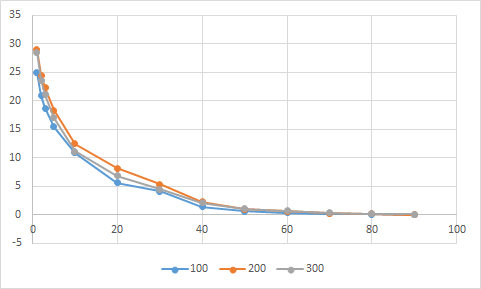
\includegraphics[scale=1]{imagenes/Experimental/DiferenciasGACEPv1.png}
        \caption{Gráfica asociada a la tabla \ref{DiferenciasGACEPv1}}
        \label{fig:DiferenciasGACEPv1}
\end{figure}

En la tabla \ref{DiferenciasGACEPv1} se puede ver que GACEP tiene un comportamiento similar con respecto a la progresión de las mejores soluciones a lo largo de la ejecución que el algoritmo base AGEU. 
Se observa que no se produce ninguna convergencia prematura, aunque es cierto que en la segunda mitad de las evaluaciones se producen muchos menos cambios que en el resto. 



\section{Uso de GRASP}

La modificación anterior tenía como objetivo aumentar la explotación de los buenos resultados. 
Para volver a conseguir un buen balance de explotación y exploración en el algoritmo lo siguiente que debemos pensar es qué clase de modificación se podría introducir de forma que aumentase la diversidad de la población y/o de las soluciones a considerar. 

La siguiente modificación que se plantea es la sustitución del uso del algoritmo Greedy por una variante suya: GRASP. 
Esta modificación solo tiene sentido usarla en el operador de reparación en la fase de aprendizaje del histórico. 
Esto es porque el único sitio donde se utiliza Greedy es en el operador de reparación, que intenta introducir siempre el mejor elemento a la solución y eliminar el peor. 
Durante la fase de acción del histórico ya realiza de por si un procedimiento similar al del GRASP \ref{alg:GRASP}, ya que le da prioridad a introducir alguno (sin comprobar si es verdaderamente el mejor) de los mejores elementos aprendidos y eliminar alguno (sin comprobar si verdaderamente es el peor) de los peores elementos aprendidos. 

El objetivo de esta modificación es introducir un operador que permita diversificar la población, eliminando el determinismo de siempre elegir las mismos elementos. 
De esta forma, somos capaces de darle más importancia a la parte de exploración del algoritmo, pero siempre manteniendo que las soluciones sigan intentando ser lo mejor posible. 

Por tanto, \textbf{GACEPv2} será resultado de añadir un operador GRASP al operador de reparación de GACEPv1.

Los resultados de la ejecución del algoritmo GACEP con esta modificación pueden verse en la tabla \ref{GACEPv2}. 

Con esto, debemos comprobar si realmente se ha producido una mejora con respecto a la modificación anterior. 
Para ello compararemos sus resultados y estableceremos un \textit{ranking}, siendo la gráfica correspondiente a esta comparación la gráfica \ref{fig:AGEUvsGACEPv1}. 


\begin{figure}[h]
     \centering
     \begin{subfigure}[b]{0.45\textwidth}
         \centering
         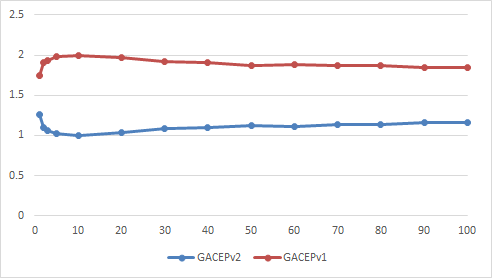
\includegraphics[width=\textwidth]{imagenes/Experimental/GRASPvswoGRASP.png}
         \caption{Ranking durante todas las \textit{milestones}}
         \label{fig:AGEUvsGACEPv1_lineas}
     \end{subfigure}
     \hfill
     \begin{subfigure}[b]{0.45\textwidth}
         \centering
         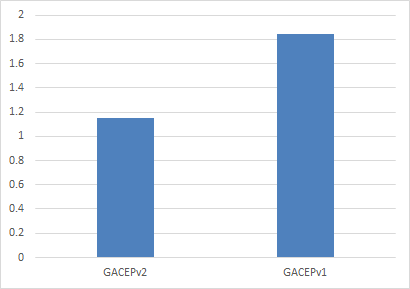
\includegraphics[width=\textwidth]{imagenes/Experimental/barras/GRASPvswoGRASP.png}
         \caption{Ranking final}
         \label{fig:AGEUvsGACEPv1_barras}
     \end{subfigure}
        \caption{Comparación de los resultados del GACEPv1 y GACEPv2}
        \label{fig:AGEUvsGACEPv1}
\end{figure}

En esta gráfica \ref{fig:AGEUvsGACEPv1} se puede ver cómo la nueva versión, introduciendo GRASP, es consistentemente mejor que la versión anterior. 
Es más, se puede afirmar que es mejor en casi todos los datos utilizados. 
Por lo tanto, se procederá a continuar con el desarrollo de nuestro algoritmo sobre esta nueva versión.

A continuación, se mostrará una tabla \ref{DiferenciasGACEP_GRASP} que almacena la media de las diferencias de los resultados de cada \textit{milestone} con respecto a la final, con el fin de comprobar si podemos sacar información sobre la convergencia de las soluciones en el tiempo. 

%GACEPv2 - Diferencias
\begin{table}[]
\begin{tabular}{|ccrccrccr|}
\hline
\rowcolor[HTML]{FFFFC7} 
\multicolumn{9}{|c|}{\cellcolor[HTML]{FFFFC7}GACEPv2}                                                                                                                                                                                                                                                                                                                                                                                                                                                                                                                     \\ \hline
\rowcolor[HTML]{F7EAC7} 
\multicolumn{1}{|c|}{\cellcolor[HTML]{F7EAC7}n}                      & \multicolumn{1}{c|}{\cellcolor[HTML]{F7EAC7}milestone} & \multicolumn{1}{l|}{\cellcolor[HTML]{F7EAC7}Diferencia} & \multicolumn{1}{c|}{\cellcolor[HTML]{F7EAC7}n}                      & \multicolumn{1}{c|}{\cellcolor[HTML]{F7EAC7}milestone} & \multicolumn{1}{l|}{\cellcolor[HTML]{F7EAC7}Diferencia} & \multicolumn{1}{c|}{\cellcolor[HTML]{F7EAC7}n}                      & \multicolumn{1}{c|}{\cellcolor[HTML]{F7EAC7}milestone} & \multicolumn{1}{l|}{\cellcolor[HTML]{F7EAC7}Diferencia} \\ \hline
\rowcolor[HTML]{DAE8FC} 
\multicolumn{1}{|c|}{\cellcolor[HTML]{FFFFC7}}                       & \multicolumn{1}{c|}{\cellcolor[HTML]{DAE8FC}1}         & \multicolumn{1}{r|}{\cellcolor[HTML]{DAE8FC}25.3737}    & \multicolumn{1}{c|}{\cellcolor[HTML]{FFFFC7}}                       & \multicolumn{1}{c|}{\cellcolor[HTML]{DAE8FC}1}         & \multicolumn{1}{r|}{\cellcolor[HTML]{DAE8FC}29.8461881} & \multicolumn{1}{c|}{\cellcolor[HTML]{FFFFC7}}                       & \multicolumn{1}{c|}{\cellcolor[HTML]{DAE8FC}1}         & 28.9145096                                              \\ \cline{2-3} \cline{5-6} \cline{8-9} 
\rowcolor[HTML]{DDFDFF} 
\multicolumn{1}{|c|}{\cellcolor[HTML]{FFFFC7}}                       & \multicolumn{1}{c|}{\cellcolor[HTML]{DDFDFF}2}         & \multicolumn{1}{r|}{\cellcolor[HTML]{DDFDFF}20.6761}    & \multicolumn{1}{c|}{\cellcolor[HTML]{FFFFC7}}                       & \multicolumn{1}{c|}{\cellcolor[HTML]{DDFDFF}2}         & \multicolumn{1}{r|}{\cellcolor[HTML]{DDFDFF}24.9678186} & \multicolumn{1}{c|}{\cellcolor[HTML]{FFFFC7}}                       & \multicolumn{1}{c|}{\cellcolor[HTML]{DDFDFF}2}         & 24.0603906                                              \\ \cline{2-3} \cline{5-6} \cline{8-9} 
\rowcolor[HTML]{DAE8FC} 
\multicolumn{1}{|c|}{\cellcolor[HTML]{FFFFC7}}                       & \multicolumn{1}{c|}{\cellcolor[HTML]{DAE8FC}3}         & \multicolumn{1}{r|}{\cellcolor[HTML]{DAE8FC}18.4198}    & \multicolumn{1}{c|}{\cellcolor[HTML]{FFFFC7}}                       & \multicolumn{1}{c|}{\cellcolor[HTML]{DAE8FC}3}         & \multicolumn{1}{r|}{\cellcolor[HTML]{DAE8FC}22.561253}  & \multicolumn{1}{c|}{\cellcolor[HTML]{FFFFC7}}                       & \multicolumn{1}{c|}{\cellcolor[HTML]{DAE8FC}3}         & 21.4992992                                              \\ \cline{2-3} \cline{5-6} \cline{8-9} 
\rowcolor[HTML]{DDFDFF} 
\multicolumn{1}{|c|}{\cellcolor[HTML]{FFFFC7}}                       & \multicolumn{1}{c|}{\cellcolor[HTML]{DDFDFF}5}         & \multicolumn{1}{r|}{\cellcolor[HTML]{DDFDFF}14.7471}    & \multicolumn{1}{c|}{\cellcolor[HTML]{FFFFC7}}                       & \multicolumn{1}{c|}{\cellcolor[HTML]{DDFDFF}5}         & \multicolumn{1}{r|}{\cellcolor[HTML]{DDFDFF}18.4329667} & \multicolumn{1}{c|}{\cellcolor[HTML]{FFFFC7}}                       & \multicolumn{1}{c|}{\cellcolor[HTML]{DDFDFF}5}         & 17.1360467                                              \\ \cline{2-3} \cline{5-6} \cline{8-9} 
\rowcolor[HTML]{DAE8FC} 
\multicolumn{1}{|c|}{\cellcolor[HTML]{FFFFC7}}                       & \multicolumn{1}{c|}{\cellcolor[HTML]{DAE8FC}10}        & \multicolumn{1}{r|}{\cellcolor[HTML]{DAE8FC}9.94967}    & \multicolumn{1}{c|}{\cellcolor[HTML]{FFFFC7}}                       & \multicolumn{1}{c|}{\cellcolor[HTML]{DAE8FC}10}        & \multicolumn{1}{r|}{\cellcolor[HTML]{DAE8FC}11.9316113} & \multicolumn{1}{c|}{\cellcolor[HTML]{FFFFC7}}                       & \multicolumn{1}{c|}{\cellcolor[HTML]{DAE8FC}10}        & 10.5285922                                              \\ \cline{2-3} \cline{5-6} \cline{8-9} 
\rowcolor[HTML]{DDFDFF} 
\multicolumn{1}{|c|}{\cellcolor[HTML]{FFFFC7}}                       & \multicolumn{1}{c|}{\cellcolor[HTML]{DDFDFF}20}        & \multicolumn{1}{r|}{\cellcolor[HTML]{DDFDFF}5.62915}    & \multicolumn{1}{c|}{\cellcolor[HTML]{FFFFC7}}                       & \multicolumn{1}{c|}{\cellcolor[HTML]{DDFDFF}20}        & \multicolumn{1}{r|}{\cellcolor[HTML]{DDFDFF}7.98414965} & \multicolumn{1}{c|}{\cellcolor[HTML]{FFFFC7}}                       & \multicolumn{1}{c|}{\cellcolor[HTML]{DDFDFF}20}        & 6.88853082                                              \\ \cline{2-3} \cline{5-6} \cline{8-9} 
\rowcolor[HTML]{DAE8FC} 
\multicolumn{1}{|c|}{\cellcolor[HTML]{FFFFC7}}                       & \multicolumn{1}{c|}{\cellcolor[HTML]{DAE8FC}30}        & \multicolumn{1}{r|}{\cellcolor[HTML]{DAE8FC}4.38901}    & \multicolumn{1}{c|}{\cellcolor[HTML]{FFFFC7}}                       & \multicolumn{1}{c|}{\cellcolor[HTML]{DAE8FC}30}        & \multicolumn{1}{r|}{\cellcolor[HTML]{DAE8FC}5.14003393} & \multicolumn{1}{c|}{\cellcolor[HTML]{FFFFC7}}                       & \multicolumn{1}{c|}{\cellcolor[HTML]{DAE8FC}30}        & 4.43403031                                              \\ \cline{2-3} \cline{5-6} \cline{8-9} 
\rowcolor[HTML]{DDFDFF} 
\multicolumn{1}{|c|}{\cellcolor[HTML]{FFFFC7}}                       & \multicolumn{1}{c|}{\cellcolor[HTML]{DDFDFF}40}        & \multicolumn{1}{r|}{\cellcolor[HTML]{DDFDFF}0.7794}     & \multicolumn{1}{c|}{\cellcolor[HTML]{FFFFC7}}                       & \multicolumn{1}{c|}{\cellcolor[HTML]{DDFDFF}40}        & \multicolumn{1}{r|}{\cellcolor[HTML]{DDFDFF}2.28877565} & \multicolumn{1}{c|}{\cellcolor[HTML]{FFFFC7}}                       & \multicolumn{1}{c|}{\cellcolor[HTML]{DDFDFF}40}        & 2.14374372                                              \\ \cline{2-3} \cline{5-6} \cline{8-9} 
\rowcolor[HTML]{DAE8FC} 
\multicolumn{1}{|c|}{\cellcolor[HTML]{FFFFC7}}                       & \multicolumn{1}{c|}{\cellcolor[HTML]{DAE8FC}50}        & \multicolumn{1}{r|}{\cellcolor[HTML]{DAE8FC}0.21656}    & \multicolumn{1}{c|}{\cellcolor[HTML]{FFFFC7}}                       & \multicolumn{1}{c|}{\cellcolor[HTML]{DAE8FC}50}        & \multicolumn{1}{r|}{\cellcolor[HTML]{DAE8FC}1.07903317} & \multicolumn{1}{c|}{\cellcolor[HTML]{FFFFC7}}                       & \multicolumn{1}{c|}{\cellcolor[HTML]{DAE8FC}50}        & 1.15285329                                              \\ \cline{2-3} \cline{5-6} \cline{8-9} 
\rowcolor[HTML]{DDFDFF} 
\multicolumn{1}{|c|}{\cellcolor[HTML]{FFFFC7}}                       & \multicolumn{1}{c|}{\cellcolor[HTML]{DDFDFF}60}        & \multicolumn{1}{r|}{\cellcolor[HTML]{DDFDFF}0.06538}    & \multicolumn{1}{c|}{\cellcolor[HTML]{FFFFC7}}                       & \multicolumn{1}{c|}{\cellcolor[HTML]{DDFDFF}60}        & \multicolumn{1}{r|}{\cellcolor[HTML]{DDFDFF}0.42600859} & \multicolumn{1}{c|}{\cellcolor[HTML]{FFFFC7}}                       & \multicolumn{1}{c|}{\cellcolor[HTML]{DDFDFF}60}        & 0.59987399                                              \\ \cline{2-3} \cline{5-6} \cline{8-9} 
\rowcolor[HTML]{DAE8FC} 
\multicolumn{1}{|c|}{\cellcolor[HTML]{FFFFC7}}                       & \multicolumn{1}{c|}{\cellcolor[HTML]{DAE8FC}70}        & \multicolumn{1}{r|}{\cellcolor[HTML]{DAE8FC}0.01904}    & \multicolumn{1}{c|}{\cellcolor[HTML]{FFFFC7}}                       & \multicolumn{1}{c|}{\cellcolor[HTML]{DAE8FC}70}        & \multicolumn{1}{r|}{\cellcolor[HTML]{DAE8FC}0.04685168} & \multicolumn{1}{c|}{\cellcolor[HTML]{FFFFC7}}                       & \multicolumn{1}{c|}{\cellcolor[HTML]{DAE8FC}70}        & 0.17475741                                              \\ \cline{2-3} \cline{5-6} \cline{8-9} 
\rowcolor[HTML]{DDFDFF} 
\multicolumn{1}{|c|}{\cellcolor[HTML]{FFFFC7}}                       & \multicolumn{1}{c|}{\cellcolor[HTML]{DDFDFF}80}        & \multicolumn{1}{r|}{\cellcolor[HTML]{DDFDFF}0.00528}    & \multicolumn{1}{c|}{\cellcolor[HTML]{FFFFC7}}                       & \multicolumn{1}{c|}{\cellcolor[HTML]{DDFDFF}80}        & \multicolumn{1}{r|}{\cellcolor[HTML]{DDFDFF}0.01998544} & \multicolumn{1}{c|}{\cellcolor[HTML]{FFFFC7}}                       & \multicolumn{1}{c|}{\cellcolor[HTML]{DDFDFF}80}        & 0.10914333                                              \\ \cline{2-3} \cline{5-6} \cline{8-9} 
\rowcolor[HTML]{DAE8FC} 
\multicolumn{1}{|c|}{\multirow{-13}{*}{\cellcolor[HTML]{FFFFC7}100}} & \multicolumn{1}{c|}{\cellcolor[HTML]{DAE8FC}90}        & \multicolumn{1}{r|}{\cellcolor[HTML]{DAE8FC}-0.0014}    & \multicolumn{1}{c|}{\multirow{-13}{*}{\cellcolor[HTML]{FFFFC7}200}} & \multicolumn{1}{c|}{\cellcolor[HTML]{DAE8FC}90}        & \multicolumn{1}{r|}{\cellcolor[HTML]{DAE8FC}0.00014457} & \multicolumn{1}{c|}{\multirow{-13}{*}{\cellcolor[HTML]{FFFFC7}300}} & \multicolumn{1}{c|}{\cellcolor[HTML]{DAE8FC}90}        & 0.00313706                                              \\ \hline
\end{tabular}
\caption{\label{DiferenciasGACEP_GRASP}Diferencias de los resultados de las distintas milestones con respecto a la final para el algoritmo GACEPv2}
\end{table}

\begin{figure}[h]
		\centering
		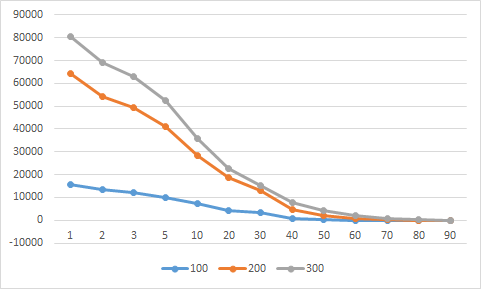
\includegraphics[scale=1]{imagenes/Experimental/DiferenciasGACEP_GRASP.png}
        \caption{Gráfica asociada a la tabla \ref{DiferenciasGACEP_GRASP}}
        \label{fig:DiferenciasGACEP}
\end{figure}

Comparando las tablas de diferencias \ref{DiferenciasGACEPv1} y \ref{DiferenciasGACEP_GRASP} se puede ver que al principio parece que sí introduce algo más de diversidad (ya que las soluciones en dichas \textit{milestones} son más diferentes a la final), aunque esto es solo notable para los tamaños $n=200$ y $n=300$. 

\section{Operador de Cruce Intensivo}

La siguiente idea a seguir tiene que ver de nuevo con la explotación de las características de las mejores soluciones. 
Anteriormente se propuso introducir una modificación para mejorar la explotación en el propio operador de reparación y en la mutación; en este caso, se pretende introducir este operador en el propio operador de cruce directamente. 

Esta modificación se basa en que las soluciones hijas heredarán una mayor cantidad de genes del mejor de los dos padres. 
La motivación de este cambio es la generación de nuevas soluciones muy parecidas a las buenas que ya forman parte de la población, con lo que hay una mayor probabilidad de que se sigan desarrollando las soluciones en ese ámbito. 

Para este trabajo probaremos con varios porcentajes de elementos que deben ser pertenecientes al mejor padre: 50\%, 60\%, 70\% y 80\%, para decidir cuál sería la mejor proporción. 
Téngase en cuenta que elegir el 50\% de los genes del mejor padre no tiene por qué tener el mismo resultado que el cruce uniforme que estamos actualmente realizando; ya que la primera opción permite que ambos hijos tengan genes en común (que provengan del mismo padre), mientras que para la segunda opción eso es imposible. 

Adicionalmente, consideraremos también dos posibilidades mayores: el utilizar GRASP de nuevo para este tipo de cruce o no. 
De antemano podríamos suponer que el uso del GRASP dará mejores resultados, ya que ayudará a diversificar unas soluciones hijas que serán muy parecidas entre sí en tanto que tomarán bastantes elementos del mismo padre. 
Pero esto debemos comprobarlo empíricamente, por ello, se calculan todos los resultados posibles y se comparan entre sí para determinar cuál es la mejor opción, la cual compararemos posteriormente con nuestro GACEPv2. 

\subsection{Utilizando GRASP}

La lógica de utilizar GRASP para el cruce intensivo es la misma que para el cruce uniforme, la utilizaremos en el operador de reparación tras generar los hijos resultantes de dicho cruce. 

Estas versiones recibirán el nombre ``\textbf{GACEPv3c\texttt{x}}'', donde \texttt{x} en este caso representaría el porcentaje de elementos que toma del mejor padre.

Dicho esto, podemos ver en la gráfica \ref{fig:GACEPcGRASP} el \textit{ranking} de los distintos porcentajes asociados al operador de cruce.

\begin{figure}[h]
     \centering
     \begin{subfigure}[b]{0.45\textwidth}
         \centering
         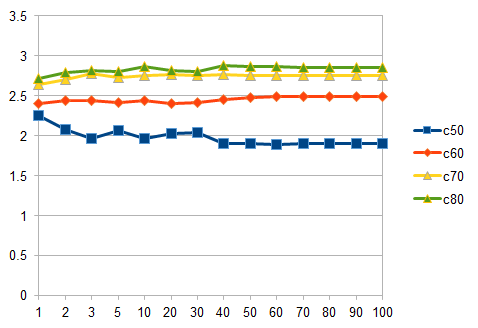
\includegraphics[width=\textwidth]{imagenes/Experimental/GACEPcGRASP.png}
         \caption{Ranking durante todas las \textit{milestones}}
         \label{fig:GACEPv3cGRASP_lineas}
     \end{subfigure}
     \hfill
     \begin{subfigure}[b]{0.45\textwidth}
         \centering
         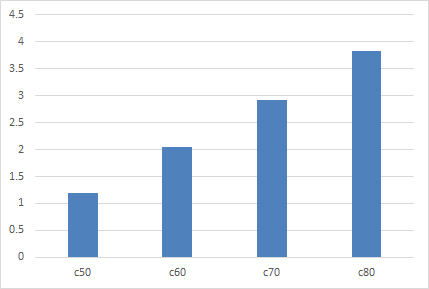
\includegraphics[width=\textwidth]{imagenes/Experimental/barras/GACEPcGRASP.png}
         \caption{Ranking final}
         \label{fig:GACEPv3cGRASP_barras}
     \end{subfigure}
        \caption{Comparación de los resultados de los GACEPv3c\texttt{x}}
        \label{fig:GACEPcGRASP}
\end{figure}

\subsection{Sin utilizar GRASP}

En este caso se seguiría usando el Operador de Reparación original (\ref{alg:OR}), donde se elige automáticamente el mejor elemento posible para introducir y el peor elemento posible para eliminar.

Estas versiones recibirán el nombre ``\textbf{GACEPv3c\texttt{x}wo}'', donde \texttt{x} en este caso representaría el porcentaje de elementos que toma del mejor padre y ``wo'' indica que no se está utilizando GRASP (\textit{without GRASP}).

En la gráfica \ref{fig:GACEPcwoGRASP} podemos apreciar el \textit{ranking} de los distintos porcentajes asociados al operador de cruce.

\begin{figure}[h]
     \centering
     \begin{subfigure}[b]{0.45\textwidth}
         \centering
         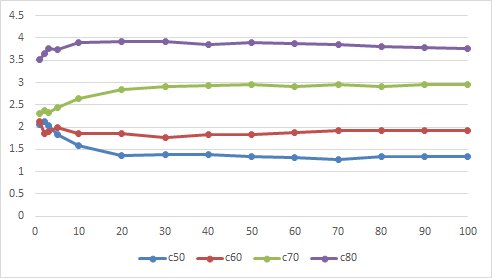
\includegraphics[width=\textwidth]{imagenes/Experimental/GACEPcwoGRASP.png}
         \caption{Ranking durante todas las \textit{milestones}}
         \label{fig:GACEPv3cwo_lineas}
     \end{subfigure}
     \hfill
     \begin{subfigure}[b]{0.45\textwidth}
         \centering
         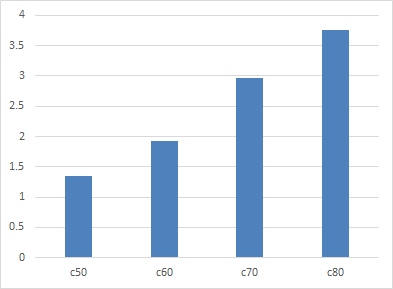
\includegraphics[width=\textwidth]{imagenes/Experimental/barras/GACEPcwoGRASP.png}
         \caption{Ranking final}
         \label{fig:GACEPv3cwo_barras}
     \end{subfigure}
        \caption{Comparación de los resultados de los GACEPv3c\texttt{x}wo}
        \label{fig:GACEPcwoGRASP}
\end{figure}

Se puede apreciar que en ambos casos, el comportamiento que tienen los algoritmos es similar, cuanta mayor sea la intensidad con la que se aplique el nuevo operador de cruce peores son los resultados. 
Con esto se puede empezar a intuir que, al menos para poblaciones pequeñas, tener muchas soluciones parecidas resulta contraproducente, ya que reduce la diversidad y llega a estancar a la población. 
Por lo tanto, procederemos a comparar las mejores versiones de ambas opciones: las dos utilizando un 50\% de los elementos del mejor padre. 
En la gráfica \ref{fig:GACEPv3c} podemos apreciar el \textit{ranking} de ambas opciones tanto para las distintas \textit{milestones} como la final sola.

\begin{figure}[h]
     \centering
     \begin{subfigure}[b]{0.45\textwidth}
         \centering
         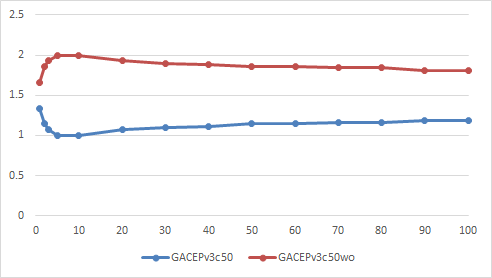
\includegraphics[width=\textwidth]{imagenes/Experimental/GACEPv3c.png}
         \caption{Ranking durante todas las \textit{milestones}}
         \label{fig:GACEPv3c_lineas}
     \end{subfigure}
     \hfill
     \begin{subfigure}[b]{0.45\textwidth}
         \centering
         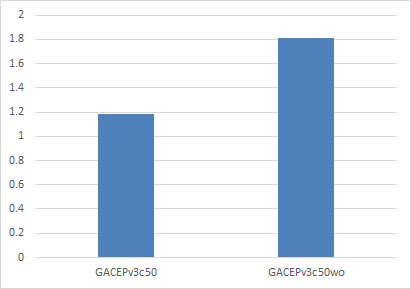
\includegraphics[width=\textwidth]{imagenes/Experimental/barras/GACEPv3c.png}
         \caption{Ranking final}
         \label{fig:GACEPv3c_barras}
     \end{subfigure}
        \caption{Comparación de los resultados de los GACEPv3c50 y GACEPv3c50wo}
        \label{fig:GACEPv3c}
\end{figure}

En \ref{fig:GACEPv3c_lineas} podemos ver que el usar la opción con GRASP es superior a la versión que no lo usa. 
Con esto podemos extraer que el uso del GRASP es adecuado para ambos operadores de cruce: el uniforme \ref{alg:CU} y el porcentual \ref{alg:CI}. 

Esto último nos lleva a tener que comparar los algoritmos GACEPv2 y GACEPv3c50 para determinar si se ha producido alguna mejora. 
Esta comparación puede ser visualizada en la gráfica \ref{fig:GACEPv2vsGACEPv3}.

\begin{figure}[h]
     \centering
     \begin{subfigure}[b]{0.45\textwidth}
         \centering
         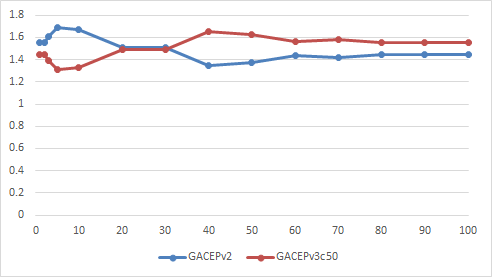
\includegraphics[width=\textwidth]{imagenes/Experimental/GACEPv2vsGACEPv3.png}
         \caption{Ranking durante todas las \textit{milestones}}
         \label{fig:GACEPv2vsGACEPv3_lineas}
     \end{subfigure}
     \hfill
     \begin{subfigure}[b]{0.45\textwidth}
         \centering
         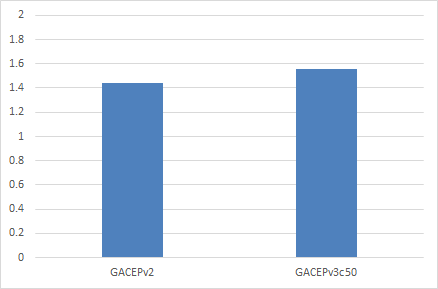
\includegraphics[width=\textwidth]{imagenes/Experimental/barras/GACEPv2vsGACEPv3.png}
         \caption{Ranking final}
         \label{fig:GACEPv2vsGACEPv3_barras}
     \end{subfigure}
        \caption{Comparación de los resultados de los GACEPv2 y GACEPv3c50}
        \label{fig:GACEPv2vsGACEPv3}
\end{figure}

En la gráfica \ref{fig:GACEPv2vsGACEPv3_lineas} que aunque en las primeras iteraciones el GACEPv3c50 tiene mejores resultados que GACEPv2, esta diferencia se reduce rápidamente. 
De hecho, las dos versiones tienen resultados muy parecidos, lo cual tiene sentido ya que el cruce uniforme y el cruce porcentual del 50\% son muy similares, aunque no iguales. 
De cualquier forma, a partir del 30\% de las iteraciones GACEPv2 obtiene mejores resultados que GACEPv3c50, aunque sea por poco. 
Por lo tanto, ignoraremos esta tercera versión y seguiremos trabajando con la segunda versión como base. 

\section{Modificaciones sobre CHC}

Llegados a este punto podemos considerar haber hecho algunos avances significativos sobre el AGEU y es momento de preguntarse si estas modificaciones se podrían aplicar al algoritmo CHC. 
Recordemos que en \ref{fig:AGEUvsCHC_lineas} podíamos apreciar que CHC obtenía mejores resultados en la primera mitad de las iteraciones y al final resultaba peor dado a que convergía prematuramente. 
Por lo tanto, en esta sección vamos a comprobar si aplicando los mismos cambios que al AGEU se logra mejorar los resultados del GACEP. 

En tanto que no es una versión puramente de GACEP, cambiaremos su notación a ``\textbf{GACEPCHCv\texttt{x}}'', donde \texttt{x} representa el número de la versión. 

\subsection{Incorporación del histórico}

El uso del histórico \ref{alg:Historico_Estructura} para CHC sigue la misma lógica que para el AGEU: el aumento de la explotación de los mejores resultados. 
Si bien a simple vista se podría pensar que el uso del histórico no debería mejorar los resultados ya que nuestro problema principal es que la población converge rápidamente a una solución se debe recordar cómo se clasificaban los distintos elementos:
\begin{itemize}
	\item \texttt{Mejores}: Aquellos elementos que suelen estar presentes en las mejores soluciones, pero no en las peores.
	\item \texttt{Peores}: Aquellos elementos que suelen estar presentes en las peores soluciones, pero no en las mejores. 
	\item \texttt{Sin información}: Aquellos elementos que frecuentemente no aparecen en las mejores ni en las peores soluciones o que aparecen en ambas (por lo que no nos aporta ninguna información ya que no se puede considerar un elemento determinista en lo buena que es una solución).
\end{itemize}
Por lo que si todas las soluciones son muy parecidas entre sí, teniendo todas el mismo conjunto de elementos, estos elementos no se considerarán ``mejores'' que el resto y tendrán la misma probabilidad de ser elegidas que el resto de elementos que no se han explorado anteriormente. 

Esta versión se denominará \textbf{GACEPCHCv1}.

Como hemos hecho previamente, obtendremos sus resultados, los cuales están almacenados en \color{red} METER TABLA EN EL APENDICE\color{black}. 
Estos resultados los compararemos con los del CHC versión \textit{expensive} para determinar si se ha producido algún tipo de mejora. 
Esta comparación será visible en la gráfica \ref{fig:CHCvsGACEPCHCv1}

\begin{figure}[h]
     \centering
     \begin{subfigure}[b]{0.45\textwidth}
         \centering
         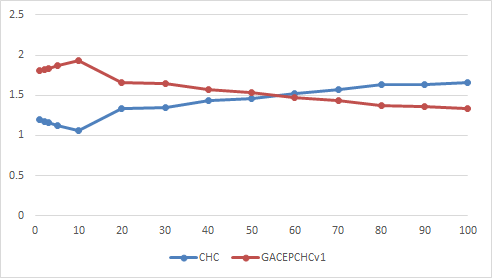
\includegraphics[width=\textwidth]{imagenes/Experimental/CHCvsGACEPCHCv1.png}
         \caption{Ranking durante todas las \textit{milestones}}
         \label{fig:CHCvsGACEPCHCv1_lineas}
     \end{subfigure}
     \hfill
     \begin{subfigure}[b]{0.45\textwidth}
         \centering
         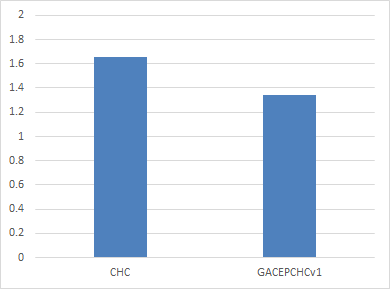
\includegraphics[width=\textwidth]{imagenes/Experimental/barras/CHCvsGACEPCHCv1.png}
         \caption{Ranking final}
         \label{fig:CHCvsGACEPCHCv1_barras}
     \end{subfigure}
        \caption{Comparación de los resultados de CHC y GACEPCHCv1}
        \label{fig:CHCvsGACEPCHCv1}
\end{figure}

En esta gráfica \ref{fig:CHCvsGACEPCHCv1} se puede apreciar que aunque inicialmente GACEPCHCv1 es bastante peor que CHC, tras la mitad de las ejecuciones logra mejorarlo. 
Esto podría estar causado por el hecho de que CHC converge rápidamente antes de la mitad de las ejecuciones y que GACEPCHCv1 puede que siga mejorando poco a poco como lo harían las versiones anteriores basadas en AGEU debido a cierto aumento de la diversidad en la población. 
Para comprobar si este es el caso, estudiaremos las diferencias entre las soluciones de las distintas \textit{milestones} y la final. 
Esta información se mostrará en la tabla y su correspondiente gráfica

%GACEPCHCv1
\begin{table}[]
\begin{tabular}{|ccrccrccr|}
\hline
\rowcolor[HTML]{FFFFC7} 
\multicolumn{9}{|c|}{\cellcolor[HTML]{FFFFC7}GACEPCHCv1}                                                                                                                                                                                                                                                                                                                                                                                                                                                                                                                                             \\ \hline
\rowcolor[HTML]{F7EAC7} 
\multicolumn{1}{|c|}{\cellcolor[HTML]{F7EAC7}n}                               & \multicolumn{1}{c|}{\cellcolor[HTML]{F7EAC7}milestone} & \multicolumn{1}{l|}{\cellcolor[HTML]{F7EAC7}Diferencia} & \multicolumn{1}{c|}{\cellcolor[HTML]{F7EAC7}n}                               & \multicolumn{1}{c|}{\cellcolor[HTML]{F7EAC7}milestone} & \multicolumn{1}{l|}{\cellcolor[HTML]{F7EAC7}Diferencia} & \multicolumn{1}{c|}{\cellcolor[HTML]{F7EAC7}n}                               & \multicolumn{1}{c|}{\cellcolor[HTML]{F7EAC7}milestone} & \multicolumn{1}{l|}{\cellcolor[HTML]{F7EAC7}Diferencia} \\ \hline
\rowcolor[HTML]{DAE8FC} 
\multicolumn{1}{|c|}{\cellcolor[HTML]{FFFFC7}}                                & \multicolumn{1}{c|}{\cellcolor[HTML]{DAE8FC}1}         & \multicolumn{1}{r|}{\cellcolor[HTML]{DAE8FC}26.7201}    & \multicolumn{1}{c|}{\cellcolor[HTML]{FFFFC7}}                                & \multicolumn{1}{c|}{\cellcolor[HTML]{DAE8FC}1}         & \multicolumn{1}{r|}{\cellcolor[HTML]{DAE8FC}25.7172359} & \multicolumn{1}{c|}{\cellcolor[HTML]{FFFFC7}}                                & \multicolumn{1}{c|}{\cellcolor[HTML]{DAE8FC}1}         & 26.2254573                                              \\ \cline{2-3} \cline{5-6} \cline{8-9} 
\rowcolor[HTML]{DDFDFF} 
\multicolumn{1}{|c|}{\cellcolor[HTML]{FFFFC7}}                                & \multicolumn{1}{c|}{\cellcolor[HTML]{DDFDFF}2}         & \multicolumn{1}{r|}{\cellcolor[HTML]{DDFDFF}23.2096}    & \multicolumn{1}{c|}{\cellcolor[HTML]{FFFFC7}}                                & \multicolumn{1}{c|}{\cellcolor[HTML]{DDFDFF}2}         & \multicolumn{1}{r|}{\cellcolor[HTML]{DDFDFF}22.3721298} & \multicolumn{1}{c|}{\cellcolor[HTML]{FFFFC7}}                                & \multicolumn{1}{c|}{\cellcolor[HTML]{DDFDFF}2}         & 22.0835516                                              \\ \cline{2-3} \cline{5-6} \cline{8-9} 
\rowcolor[HTML]{DAE8FC} 
\multicolumn{1}{|c|}{\cellcolor[HTML]{FFFFC7}}                                & \multicolumn{1}{c|}{\cellcolor[HTML]{DAE8FC}3}         & \multicolumn{1}{r|}{\cellcolor[HTML]{DAE8FC}21.5554}    & \multicolumn{1}{c|}{\cellcolor[HTML]{FFFFC7}}                                & \multicolumn{1}{c|}{\cellcolor[HTML]{DAE8FC}3}         & \multicolumn{1}{r|}{\cellcolor[HTML]{DAE8FC}20.5934122} & \multicolumn{1}{c|}{\cellcolor[HTML]{FFFFC7}}                                & \multicolumn{1}{c|}{\cellcolor[HTML]{DAE8FC}3}         & 20.2131967                                              \\ \cline{2-3} \cline{5-6} \cline{8-9} 
\rowcolor[HTML]{DDFDFF} 
\multicolumn{1}{|c|}{\cellcolor[HTML]{FFFFC7}}                                & \multicolumn{1}{c|}{\cellcolor[HTML]{DDFDFF}5}         & \multicolumn{1}{r|}{\cellcolor[HTML]{DDFDFF}18.774}     & \multicolumn{1}{c|}{\cellcolor[HTML]{FFFFC7}}                                & \multicolumn{1}{c|}{\cellcolor[HTML]{DDFDFF}5}         & \multicolumn{1}{r|}{\cellcolor[HTML]{DDFDFF}17.9674193} & \multicolumn{1}{c|}{\cellcolor[HTML]{FFFFC7}}                                & \multicolumn{1}{c|}{\cellcolor[HTML]{DDFDFF}5}         & 17.375892                                               \\ \cline{2-3} \cline{5-6} \cline{8-9} 
\rowcolor[HTML]{DAE8FC} 
\multicolumn{1}{|c|}{\cellcolor[HTML]{FFFFC7}}                                & \multicolumn{1}{c|}{\cellcolor[HTML]{DAE8FC}10}        & \multicolumn{1}{r|}{\cellcolor[HTML]{DAE8FC}14.7039}    & \multicolumn{1}{c|}{\cellcolor[HTML]{FFFFC7}}                                & \multicolumn{1}{c|}{\cellcolor[HTML]{DAE8FC}10}        & \multicolumn{1}{r|}{\cellcolor[HTML]{DAE8FC}13.6488991} & \multicolumn{1}{c|}{\cellcolor[HTML]{FFFFC7}}                                & \multicolumn{1}{c|}{\cellcolor[HTML]{DAE8FC}10}        & 12.7586834                                              \\ \cline{2-3} \cline{5-6} \cline{8-9} 
\rowcolor[HTML]{DDFDFF} 
\multicolumn{1}{|c|}{\cellcolor[HTML]{FFFFC7}}                                & \multicolumn{1}{c|}{\cellcolor[HTML]{DDFDFF}20}        & \multicolumn{1}{r|}{\cellcolor[HTML]{DDFDFF}5.48547}    & \multicolumn{1}{c|}{\cellcolor[HTML]{FFFFC7}}                                & \multicolumn{1}{c|}{\cellcolor[HTML]{DDFDFF}20}        & \multicolumn{1}{r|}{\cellcolor[HTML]{DDFDFF}4.77580753} & \multicolumn{1}{c|}{\cellcolor[HTML]{FFFFC7}}                                & \multicolumn{1}{c|}{\cellcolor[HTML]{DDFDFF}20}        & 4.55863648                                              \\ \cline{2-3} \cline{5-6} \cline{8-9} 
\rowcolor[HTML]{DAE8FC} 
\multicolumn{1}{|c|}{\cellcolor[HTML]{FFFFC7}}                                & \multicolumn{1}{c|}{\cellcolor[HTML]{DAE8FC}30}        & \multicolumn{1}{r|}{\cellcolor[HTML]{DAE8FC}4.59547}    & \multicolumn{1}{c|}{\cellcolor[HTML]{FFFFC7}}                                & \multicolumn{1}{c|}{\cellcolor[HTML]{DAE8FC}30}        & \multicolumn{1}{r|}{\cellcolor[HTML]{DAE8FC}4.01781911} & \multicolumn{1}{c|}{\cellcolor[HTML]{FFFFC7}}                                & \multicolumn{1}{c|}{\cellcolor[HTML]{DAE8FC}30}        & 3.702351                                                \\ \cline{2-3} \cline{5-6} \cline{8-9} 
\rowcolor[HTML]{DDFDFF} 
\multicolumn{1}{|c|}{\cellcolor[HTML]{FFFFC7}}                                & \multicolumn{1}{c|}{\cellcolor[HTML]{DDFDFF}40}        & \multicolumn{1}{r|}{\cellcolor[HTML]{DDFDFF}2.47563}    & \multicolumn{1}{c|}{\cellcolor[HTML]{FFFFC7}}                                & \multicolumn{1}{c|}{\cellcolor[HTML]{DDFDFF}40}        & \multicolumn{1}{r|}{\cellcolor[HTML]{DDFDFF}2.54730194} & \multicolumn{1}{c|}{\cellcolor[HTML]{FFFFC7}}                                & \multicolumn{1}{c|}{\cellcolor[HTML]{DDFDFF}40}        & 2.39425407                                              \\ \cline{2-3} \cline{5-6} \cline{8-9} 
\rowcolor[HTML]{DAE8FC} 
\multicolumn{1}{|c|}{\cellcolor[HTML]{FFFFC7}}                                & \multicolumn{1}{c|}{\cellcolor[HTML]{DAE8FC}50}        & \multicolumn{1}{r|}{\cellcolor[HTML]{DAE8FC}1.75038}    & \multicolumn{1}{c|}{\cellcolor[HTML]{FFFFC7}}                                & \multicolumn{1}{c|}{\cellcolor[HTML]{DAE8FC}50}        & \multicolumn{1}{r|}{\cellcolor[HTML]{DAE8FC}1.97120082} & \multicolumn{1}{c|}{\cellcolor[HTML]{FFFFC7}}                                & \multicolumn{1}{c|}{\cellcolor[HTML]{DAE8FC}50}        & 1.90218522                                              \\ \cline{2-3} \cline{5-6} \cline{8-9} 
\rowcolor[HTML]{DDFDFF} 
\multicolumn{1}{|c|}{\cellcolor[HTML]{FFFFC7}}                                & \multicolumn{1}{c|}{\cellcolor[HTML]{DDFDFF}60}        & \multicolumn{1}{r|}{\cellcolor[HTML]{DDFDFF}1.14161}    & \multicolumn{1}{c|}{\cellcolor[HTML]{FFFFC7}}                                & \multicolumn{1}{c|}{\cellcolor[HTML]{DDFDFF}60}        & \multicolumn{1}{r|}{\cellcolor[HTML]{DDFDFF}1.35810173} & \multicolumn{1}{c|}{\cellcolor[HTML]{FFFFC7}}                                & \multicolumn{1}{c|}{\cellcolor[HTML]{DDFDFF}60}        & 1.29008322                                              \\ \cline{2-3} \cline{5-6} \cline{8-9} 
\rowcolor[HTML]{DAE8FC} 
\multicolumn{1}{|c|}{\cellcolor[HTML]{FFFFC7}}                                & \multicolumn{1}{c|}{\cellcolor[HTML]{DAE8FC}70}        & \multicolumn{1}{r|}{\cellcolor[HTML]{DAE8FC}0.62625}    & \multicolumn{1}{c|}{\cellcolor[HTML]{FFFFC7}}                                & \multicolumn{1}{c|}{\cellcolor[HTML]{DAE8FC}70}        & \multicolumn{1}{r|}{\cellcolor[HTML]{DAE8FC}0.82009965} & \multicolumn{1}{c|}{\cellcolor[HTML]{FFFFC7}}                                & \multicolumn{1}{c|}{\cellcolor[HTML]{DAE8FC}70}        & 0.81355995                                              \\ \cline{2-3} \cline{5-6} \cline{8-9} 
\rowcolor[HTML]{DDFDFF} 
\multicolumn{1}{|c|}{\cellcolor[HTML]{FFFFC7}}                                & \multicolumn{1}{c|}{\cellcolor[HTML]{DDFDFF}80}        & \multicolumn{1}{r|}{\cellcolor[HTML]{DDFDFF}0.44086}    & \multicolumn{1}{c|}{\cellcolor[HTML]{FFFFC7}}                                & \multicolumn{1}{c|}{\cellcolor[HTML]{DDFDFF}80}        & \multicolumn{1}{r|}{\cellcolor[HTML]{DDFDFF}0.55229199} & \multicolumn{1}{c|}{\cellcolor[HTML]{FFFFC7}}                                & \multicolumn{1}{c|}{\cellcolor[HTML]{DDFDFF}80}        & 0.54620318                                              \\ \cline{2-3} \cline{5-6} \cline{8-9} 
\rowcolor[HTML]{DAE8FC} 
\multicolumn{1}{|c|}{\multirow{-13}{*}{\cellcolor[HTML]{FFFFC7}\textbf{100}}} & \multicolumn{1}{c|}{\cellcolor[HTML]{DAE8FC}90}        & \multicolumn{1}{r|}{\cellcolor[HTML]{DAE8FC}0.00726}    & \multicolumn{1}{c|}{\multirow{-13}{*}{\cellcolor[HTML]{FFFFC7}\textbf{200}}} & \multicolumn{1}{c|}{\cellcolor[HTML]{DAE8FC}90}        & \multicolumn{1}{r|}{\cellcolor[HTML]{DAE8FC}0.01307933} & \multicolumn{1}{c|}{\multirow{-13}{*}{\cellcolor[HTML]{FFFFC7}\textbf{300}}} & \multicolumn{1}{c|}{\cellcolor[HTML]{DAE8FC}90}        & 0.03623624                                              \\ \hline
\end{tabular}
\caption{\label{DiferenciasGACEPCHCv1}Diferencias de los resultados de las distintas milestones con respecto a la final para el algoritmo GACEPCHCv1}
\end{table}

\begin{figure}[h]
		\centering
		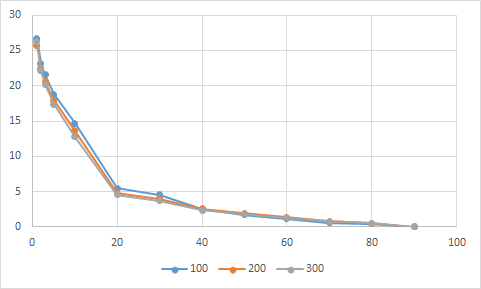
\includegraphics[scale=1]{imagenes/Experimental/DiferenciasGACEPCHCv1.png}
        \caption{Gráfica asociada a la tabla \ref{DiferenciasGACEPCHCv1}}
        \label{fig:DiferenciasGACEPCHCv1}
\end{figure}

Efectivamente, en la gráfica \ref{fig:DiferenciasGACEPCHCv1} se puede comprobar visualmente que tiene un comportamiento parecido al de las versiones de AGEU, aunque bien es verdad que es bastante más abrupto.

\subsection{Uso del GRASP}

Nuestro objetivo sigue siendo aumentar la exploración del algoritmo para conseguir una población aún más diversa y que las soluciones no converjan de forma prematura. 
Por ello se considera que este algoritmo se podría beneficiar en gran medida del uso del GRASP, podremos mantener la diversidad de la población a lo largo de la ejecución del algoritmo y, a la vez, se garantiza que las soluciones seguirán siendo competentes. 

Esta nueva versión está construida usando GACEPCHCv1 de base y la denominaremos \textbf{GACEPCHCv2}.

Tras su implementación, debemos recoger sus resultados, los cuales están almacenados en la tabla \color{red}METER TABLA EN EL APENDICE\color{black}. 
Tras esto, en primer lugar compararemos GACEPCHCv1 y GACEPCHCv2 para comprobar que realmente se ha producido una mejora de los resultados con respecto a la versión anterior. 
Esta comparación será visible en la gráfica \ref{fig:GACEPCHCv1vsGACEPCHCv2}.

\begin{figure}[h]
     \centering
     \begin{subfigure}[b]{0.45\textwidth}
         \centering
         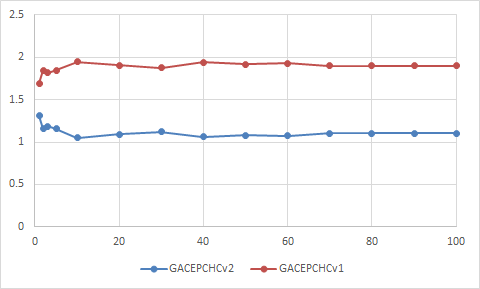
\includegraphics[width=\textwidth]{imagenes/Experimental/GACEPCHCv1vsGACEPCHCv2.png}
         \caption{Ranking durante todas las \textit{milestones}}
         \label{fig:GACEPCHCv1vsGACEPCHCv2_lineas}
     \end{subfigure}
     \hfill
     \begin{subfigure}[b]{0.45\textwidth}
         \centering
         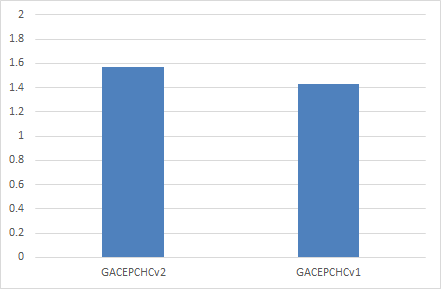
\includegraphics[width=\textwidth]{imagenes/Experimental/barras/GACEPCHCv1vsGACEPCHCv2.png}
         \caption{Ranking final}
         \label{fig:GACEPCHCv1vsGACEPCHCv2_barras}
     \end{subfigure}
        \caption{Comparación de los resultados de GACEPCHCv1 y GACEPCHCv2}
        \label{fig:GACEPCHCv1vsGACEPCHCv2}
\end{figure}

En esta gráfica \ref{fig:GACEPCHCv1vsGACEPCHCv2} podemos comprobar que efectivamente se produce una mejora con respecto a la versión anterior. 
Por lo que podemos proceder a realizar una comparación con la versión equivalente para el algoritmo AGEU: GACEPv2. 
Esta comparación será visible en la gráfica \ref{fig:GACEPv2vsGACEPCHCv2}.

\begin{figure}[h]
     \centering
     \begin{subfigure}[b]{0.45\textwidth}
         \centering
         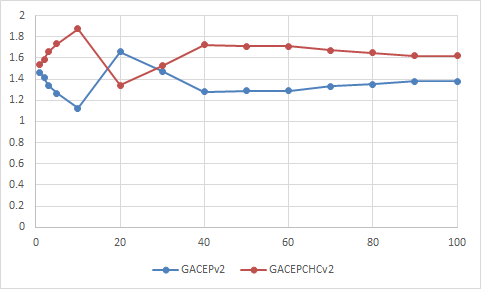
\includegraphics[width=\textwidth]{imagenes/Experimental/GACEPv2vsGACEPCHCv2.png}
         \caption{Ranking durante todas las \textit{milestones}}
         \label{fig:GACEPv2vsGACEPCHCv2_lineas}
     \end{subfigure}
     \hfill
     \begin{subfigure}[b]{0.45\textwidth}
         \centering
         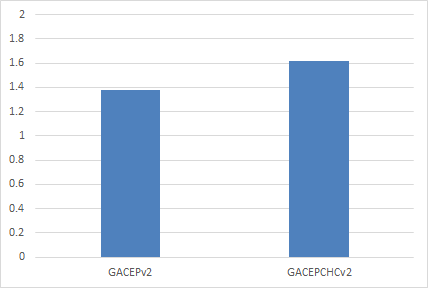
\includegraphics[width=\textwidth]{imagenes/Experimental/barras/GACEPv2vsGACEPCHCv2.png}
         \caption{Ranking final}
         \label{fig:GACEPv2vsGACEPCHCv2_barras}
     \end{subfigure}
        \caption{Comparación de los resultados de GACEPv2 y GACEPCHCv2}
        \label{fig:GACEPv2vsGACEPCHCv2}
\end{figure}

En la gráfica \ref{fig:GACEPv2vsGACEPCHCv2} se puede ver cómo GACEPv2 obtiene mejores resultados que GACEPCHCv2 en la mayoría de las \textit{milestones}, sobre todo y más importante, obtiene mejores resultados finales. 
En tanto que no se ha logrado mejorar los resultados de una versión anterior, descartaremos estos cambios y seguiremos trabajando exclusivamente sobre el algoritmo GACEPv2.

\section{Estudio de la diversidad}

\color{red}
Para poner las tablas de diversidad calculada como la diferencia entre las distintas soluciones de la población en las distintas milestones tendría que volver a ejecutarlo. 

De todas formas, el estudio se puede resumir a que hemos estado comentando que nuestras soluciones parece que ya se encuentran muy cerca de la final durante la algo más de la mitad de las iteraciones, así que realizamos propiamente un estudio de la diversidad -> Insertamos tabla + gráfica asociada -> Efectivamente hay poca diversidad, lo que nos va a llevar a implementar una serie de modificaciones dedicadas especialmente a mantener la diversidad de la población 
\color{black}

\section{Incrementando la diversidad}

Con motivo del estudio realizado en la sección anterior, resulta necesario introducir modificaciones que sean capaces de introducir y/o mantener diversidad en la población. 
En este trabajo se proponen algunas modificaciones, las cuales se explicarán individualmente y qué sentido podría tener combinarlas, comparándolas con el algoritmo GACEPv2. 
Finalmente, compararemos todas las versiones de esta sección entre sí para determinar cuál es la mejor y presentaremos como la versión final de este desarrollo. 

Un resumen de las modificaciones que aplicaremos a continuación es:
\begin{itemize}
	\item Población inicial diversa \ref{alg:PD}: Nos aseguramos que la población inicial cumpla una condición de diversidad. 
	\item Una versión del operador NAM \ref{alg:NAM}: Alteramos la elección de los padres que se utilizarán para el cruce.
	\item Una versión del \textit{Crowding} Determinístico \ref{alg:ORC}: Modificamos el operador de reemplazo.
\end{itemize}

\subsection{Población Inicial Diversa}

La motivación de esta modificación es asegurar que vamos tenemos con una población lo suficientemente diversa antes de empezar la ejecución del propio algoritmo. 
La generación de esta población inicial no computa para el número máximo de iteraciones, ya que no nos interesa saber si estas soluciones son buenas o no, solo nos interesa saber que son lo suficientemente distintas. 

Consideramos que una población será lo suficientemente diversa cuando cada una de las soluciones que la conforman difiere del resto de soluciones en al menos un \texttt{x}\% de las variables con las que tratamos. 
Se iba a realizar un estudio individual para averiguar cuál sería un \texttt{x} adecuado, sin embargo, el máximo valor que pudimos ejecutar fue \texttt{x}$=5$, ya que para valores superiores había archivos en los que era incapaz de encontrar un conjunto de soluciones que satisficiese dichas condiciones. 

Por lo tanto, para este trabajo, consideramos que una población es lo suficientemente diversa cuando cada una de las soluciones difiere del resto en, al menos, un $5\%$ de las variables que la componen. 

Esta versión tomará el nombre de \textbf{GACEPv4}. 
Los resultados de este algoritmo se encuentran en la Tabla \color{red}METER TABLA EN APÉNDICE\color{black}.

El algoritmo con esta modificación podría no considerarse una versión en sí misma, sino más bien como un prerrequisito para el resto de modificaciones de esta sección. 
Esto se debe a que la sola modificación de la población inicial no es algo que el algoritmo pueda aprovechar de forma recursiva, es solo una pequeña modificación que se hace al principio para establecer una determinada población. 
Por lo que su resultado no puede diferir mucho con respecto al de GACEPv2, como se puede apreciar en la gráfica \ref{fig:GACEPv2vsGACEPv5} (nótese la escala en la que se encuentra el eje Y en \ref{fig:GACEPv2vsGACEPv4_lineas}). 

\begin{figure}[h]
     \centering
     \begin{subfigure}[b]{0.45\textwidth}
         \centering
         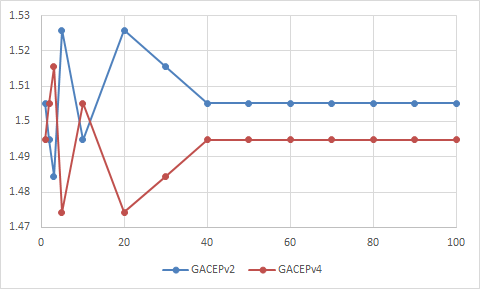
\includegraphics[width=\textwidth]{imagenes/Experimental/GACEPv2vsGACEPv4.png}
         \caption{Ranking durante todas las \textit{milestones}}
         \label{fig:GACEPv2vsGACEPv4_lineas}
     \end{subfigure}
     \hfill
     \begin{subfigure}[b]{0.45\textwidth}
         \centering
         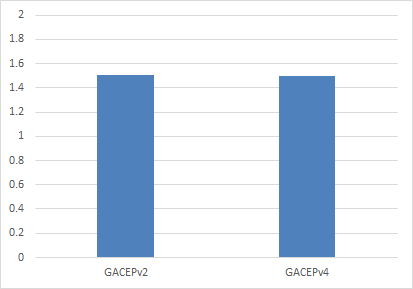
\includegraphics[width=\textwidth]{imagenes/Experimental/barras/GACEPv2vsGACEPv4.png}
         \caption{Ranking final}
         \label{fig:GACEPv2vsGACEPv4_barras}
     \end{subfigure}
        \caption{Comparación de los resultados de GACEPv2 y GACEPv4}
        \label{fig:GACEPv2vsGACEPv4}
\end{figure}

\subsection{Versión del NAM}

La motivación de esta modificación es que el cruce de dos padres lo suficientemente diferentes dará probablemente lugar a un par de soluciones que sean diferentes de ambos padres. 
En esta versión del NAM elegimos el primer padre mediante un Torneo Binario, para garantizar cierta bondad, y el segundo padre mediante el método original: escoger un subconjunto de la población y elegir como padre aquella solución más diferente al primer padre. 
Para esta modificación no hay ningún tipo de umbral de diferencias que se deba pasar para elegir al segundo padre, solo que sea lo más distinto posible. 

Esta versión tomará el nombre de \textbf{GACEPv5}. 

Esta versión ya si supone una gran modificación del propio algoritmo, por lo que es necesario obtener sus resultados \color{red} METER TABLA EN APÉNDICE \color{black} y compararlos con GACEPv2 para determinar si supone una mejora. 
Esta comparación es visible en la gráfica \ref{fig:GACEPv2vsGACEPv5}.

\begin{figure}[h]
     \centering
     \begin{subfigure}[b]{0.45\textwidth}
         \centering
         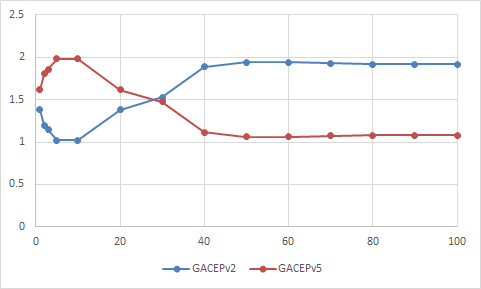
\includegraphics[width=\textwidth]{imagenes/Experimental/GACEPv2vsGACEPv5.png}
         \caption{Ranking durante todas las \textit{milestones}}
         \label{fig:GACEPv2vsGACEPv5_lineas}
     \end{subfigure}
     \hfill
     \begin{subfigure}[b]{0.45\textwidth}
         \centering
         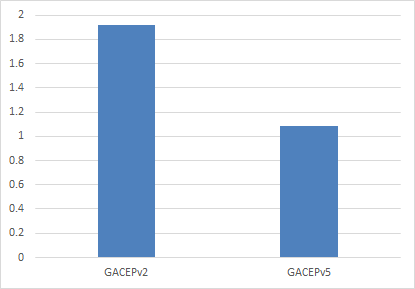
\includegraphics[width=\textwidth]{imagenes/Experimental/barras/GACEPv2vsGACEPv5.png}
         \caption{Ranking final}
         \label{fig:GACEPv2vsGACEPv5_barras}
     \end{subfigure}
        \caption{Comparación de los resultados de GACEPv2 y GACEPv5}
        \label{fig:GACEPv2vsGACEPv5}
\end{figure}

En la gráfica \ref{fig:GACEPv2vsGACEPv5_lineas} se puede ver que, aunque GACEPv2 obtiene resultados mejores en prácticamente todos los casos probados, a partir del 40\% de las ejecuciones se tiene que GACEPv5 mejora a GACEPv2 en casi todas las instancias del problema probadas. 
Por lo tanto, podemos declarar que esta modificación supone una mejora. 

\subsection{Versión del \textit{Crowding} Determinístico}

La motivación de esta modificación es que el criterio para determinar si una nueva solución se introduce o no en la población no sea únicamente el valor de dicha solución, si no también tener en cuenta si aporta diversidad. 
Es decir, dada una solución nueva se deberá buscar en primer lugar aquella solución en la población con la que más parecido tenga y la sustituirá si, y solo si, la supera en valor. 

Esta versión tomará el nombre de \textbf{GACEPv6}. 

De la misma forma que con la introducción del NAM, esta versión supone una gran modificación del propio algoritmo, por lo que es necesario obtener sus resultados \color{red} METER TABLA EN APÉNDICE \color{black} y compararlos con GACEPv2 para determinar si se ha producido una mejora. 
Esta comparación es visible en la gráfica \ref{fig:GACEPv2vsGACEPv6}.

\begin{figure}[h]
     \centering
     \begin{subfigure}[b]{0.45\textwidth}
         \centering
         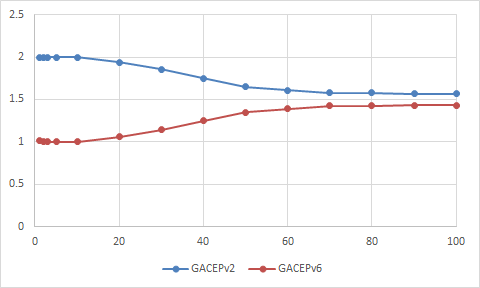
\includegraphics[width=\textwidth]{imagenes/Experimental/GACEPv2vsGACEPv6.png}
         \caption{Ranking durante todas las \textit{milestones}}
         \label{fig:GACEPv2vsGACEPv6_lineas}
     \end{subfigure}
     \hfill
     \begin{subfigure}[b]{0.45\textwidth}
         \centering
         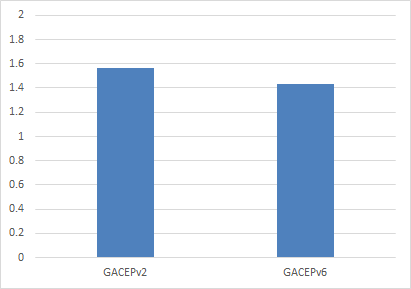
\includegraphics[width=\textwidth]{imagenes/Experimental/barras/GACEPv2vsGACEPv6.png}
         \caption{Ranking final}
         \label{fig:GACEPv2vsGACEPv6_barras}
     \end{subfigure}
        \caption{Comparación de los resultados de GACEPv2 y GACEPv6}
        \label{fig:GACEPv2vsGACEPv6}
\end{figure}

En la gráfica \ref{fig:GACEPv2vsGACEPv6_lineas} se puede comprobar que la nueva versión es mejor en todas las \textit{milestones} que GACEPv2. 
Sin embargo, es importante notar que solo se obtienen mejoras significantes durante la primera mitad de las iteraciones. 


\subsubsection{Reemplazo intensivo}

Esta versión \ref{alg:ORCv} intensifica la idea anterior, ya que no solo podrá sustituir a la solución más cercana, sino que en caso de que lo haga, se llevará un proceso de búsqueda en la población de soluciones tengan menos de cierta cantidad de diferencias con la nueva solución y nos quedaremos únicamente con aquella que sea mejor que el resto. 
En tanto que el tamaño de la población debe ser constante, el resto de soluciones serán sustituidas por soluciones generadas aleatoriamente. 
Nótese que dicho umbral de diferencia va a ser el mismo que se ha aplicado para generar una población inicial diversa y que las soluciones generadas aleatoriamente también deberán cumplir que sean lo suficientemente diversas con respecto a la población en las que son introducidas. 

Esta versión tomará el nombre de \textbf{GACEPv7}. 

En tanto que es una modificación directa sobre GACEPv6, debemos comprobar primero si se consiguen mejorar los resultados sobre esta versión. 
Los resultados obtenidos de la ejecución de GACEPv7 se pueden encontrar en la tabla \color{red} METER TABLA EN APÉNDICE \color{black} y su comparación con los resultados de GACEPv6 se puede visualizar en la gráfica \ref{fig:GACEPv6vsGACEPv7} (se ha cambiado el formato de las gráficas para una mejor visualización).

\begin{figure}[h]
		\centering
		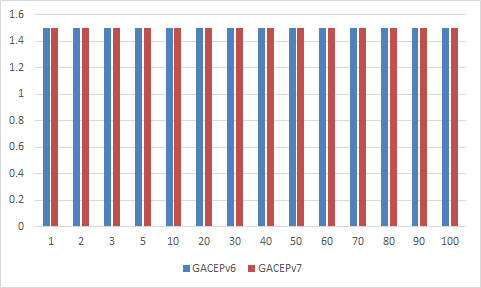
\includegraphics[scale=1]{imagenes/Experimental/barras/GACEPv6vsGACEPv7.png}
        \caption{Comparación de los resultados de GACEPv6 y GACEPv7}
        \label{fig:GACEPv6vsGACEPv7}
\end{figure}

Como se puede observar en la gráfica \ref{fig:GACEPv6vsGACEPv7}, ambas versiones dan exactamente los mismos resultados en todo momento. 
De hecho, tras obtener estos resultados se realizó un estudio de cuál era la causa y resultó que por cada hijo que se iba a introducir en la población había una o ninguna solución existente en la población dentro de este umbral, por lo que el número de soluciones a comprobar siempre era constante: una. 
Ya que incluso si no hay ninguna solución en dicho umbral, por la versión anterior se debe elegir aquella con mayor parecido para compararlas. 
Por lo tanto, esta última modificación nunca se aplicaba. 
Si bien no se ha producido ninguna mejora y descartaremos esta versión, esto nos ha ayudado a descubrir que de cierta forma se está manteniendo cierta diversidad en la población, que era el objetivo de esta sección. 

\subsection{Combinaciones}

Para este apartado, para simplificar la notación que podría llegar a tener el nombre de los algoritmos de las distintas combinaciones, estableceremos que se denominarán ``\textbf{GACEPv\texttt{xy}}'', donde \texttt{x}, \texttt{y} son dos versiones distintas de las introducidas en esta sección. 

En esta sección se han obtenido resultados bastante prometedores que en todos casos mejora a su algoritmo base, GACEPv2. 
Por lo que ahora procederemos a analizar posibles combinaciones de dichas modificaciones por si pudiesen mejorar los resultados actuales obtenidos usando GACEPv2. 

\subsubsection{GACEPv35}

En primer lugar, volvemos a considerar la posibilidad de usar un operador de cruce intensivo, dado establecimos la posibilidad de que su aplicación no aportaba buenos resultados debido a la falta de diversidad. 
En tanto que con estas nuevas modificaciones conseguimos aumentar la diversidad, es una buena idea probar de nuevo su comportamiento junto con la adición de la versión del operador NAM. 

En la gráfica \ref{fig:GACEPv35} se puede observar el comportamiento de esta nueva versión para los distintos porcentajes.
 
\begin{figure}[h]
     \centering
     \begin{subfigure}[b]{0.45\textwidth}
         \centering
         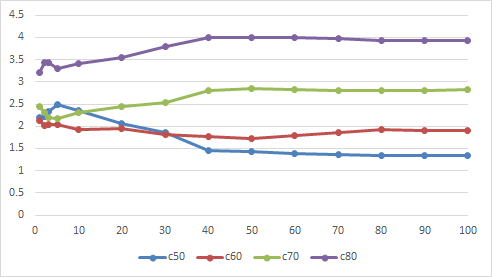
\includegraphics[width=\textwidth]{imagenes/Experimental/GACEPv35.png}
         \caption{Ranking durante todas las \textit{milestones}}
         \label{fig:GACEPv35_lineas}
     \end{subfigure}
     \hfill
     \begin{subfigure}[b]{0.45\textwidth}
         \centering
         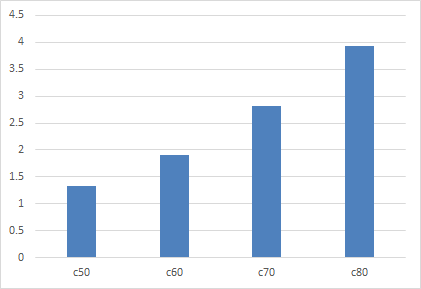
\includegraphics[width=\textwidth]{imagenes/Experimental/barras/GACEPv35.png}
         \caption{Ranking final}
         \label{fig:GACEPv35_barras}
     \end{subfigure}
        \caption{Comparación de los resultados de los GACEPv35c\texttt{x}}
        \label{fig:GACEPv35}
\end{figure}

\subsubsection{GACEPv36}

\begin{figure}[h]
     \centering
     \begin{subfigure}[b]{0.45\textwidth}
         \centering
         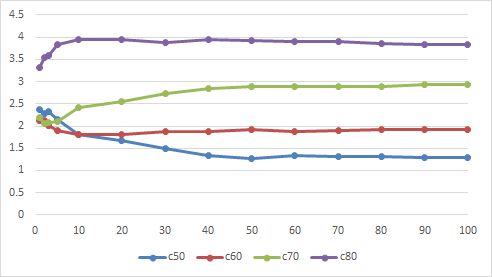
\includegraphics[width=\textwidth]{imagenes/Experimental/GACEPv36.png}
         \caption{Ranking durante todas las \textit{milestones}}
         \label{fig:GACEPv36_lineas}
     \end{subfigure}
     \hfill
     \begin{subfigure}[b]{0.45\textwidth}
         \centering
         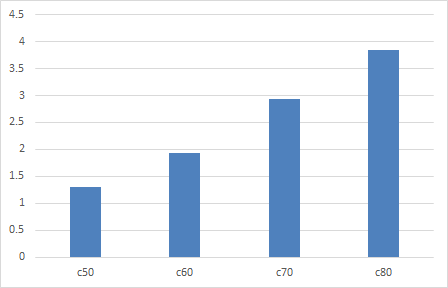
\includegraphics[width=\textwidth]{imagenes/Experimental/barras/GACEPv36.png}
         \caption{Ranking final}
         \label{fig:GACEPv36_barras}
     \end{subfigure}
        \caption{Comparación de los resultados de los GACEPv36c\texttt{x}}
        \label{fig:GACEPv36}
\end{figure}

\subsubsection{GACEPv56}

\subsubsection{GACEPv356}

\begin{figure}[h]
     \centering
     \begin{subfigure}[b]{0.45\textwidth}
         \centering
         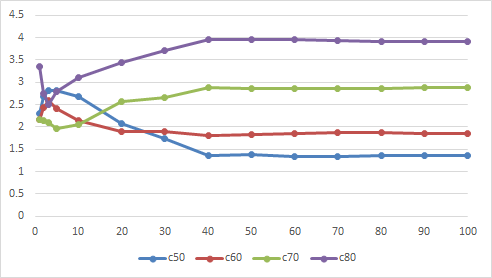
\includegraphics[width=\textwidth]{imagenes/Experimental/GACEPv356.png}
         \caption{Ranking durante todas las \textit{milestones}}
         \label{fig:GACEPv356_lineas}
     \end{subfigure}
     \hfill
     \begin{subfigure}[b]{0.45\textwidth}
         \centering
         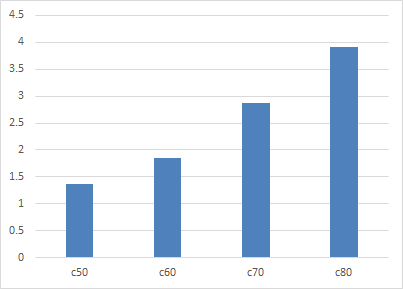
\includegraphics[width=\textwidth]{imagenes/Experimental/barras/GACEPv356.png}
         \caption{Ranking final}
         \label{fig:GACEPv356_barras}
     \end{subfigure}
        \caption{Comparación de los resultados de los GACEPv356c\texttt{x}}
        \label{fig:GACEPv356}
\end{figure}

\subsection{Comparaciones}

\section{Resumen de las versiones}

A modo de resumen de este capítulo, reuniremos todas las versiones mencionadas en una tabla
